\begin{appendices}

\chapter{Description du sujet}
\label{appendix:description}

\begin{figure}[h]
  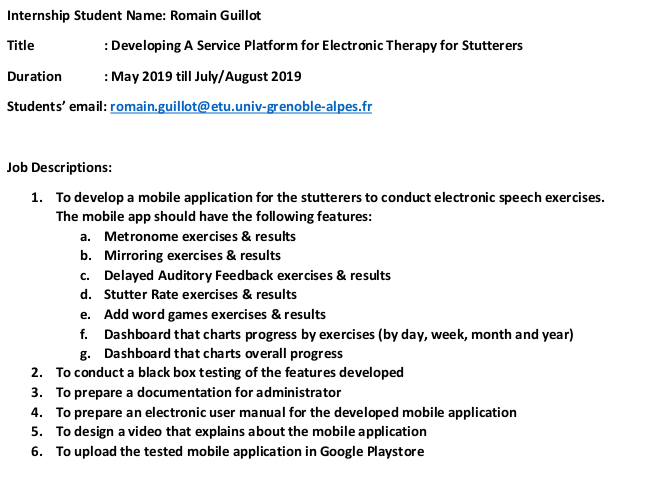
\includegraphics[width=1\linewidth]{content/imgs/description.png}
  \caption*{Description du projet proposé par ma tutrice Dr Noreen Izza Arshad}
\end{figure}


\begin{landscape}
\chapter{Stutter Manager v3}
\label{appendix:old_app}

\begin{figure}[h]
  \centering
  \begin{subfigure}{.25\textwidth}
    \centering
    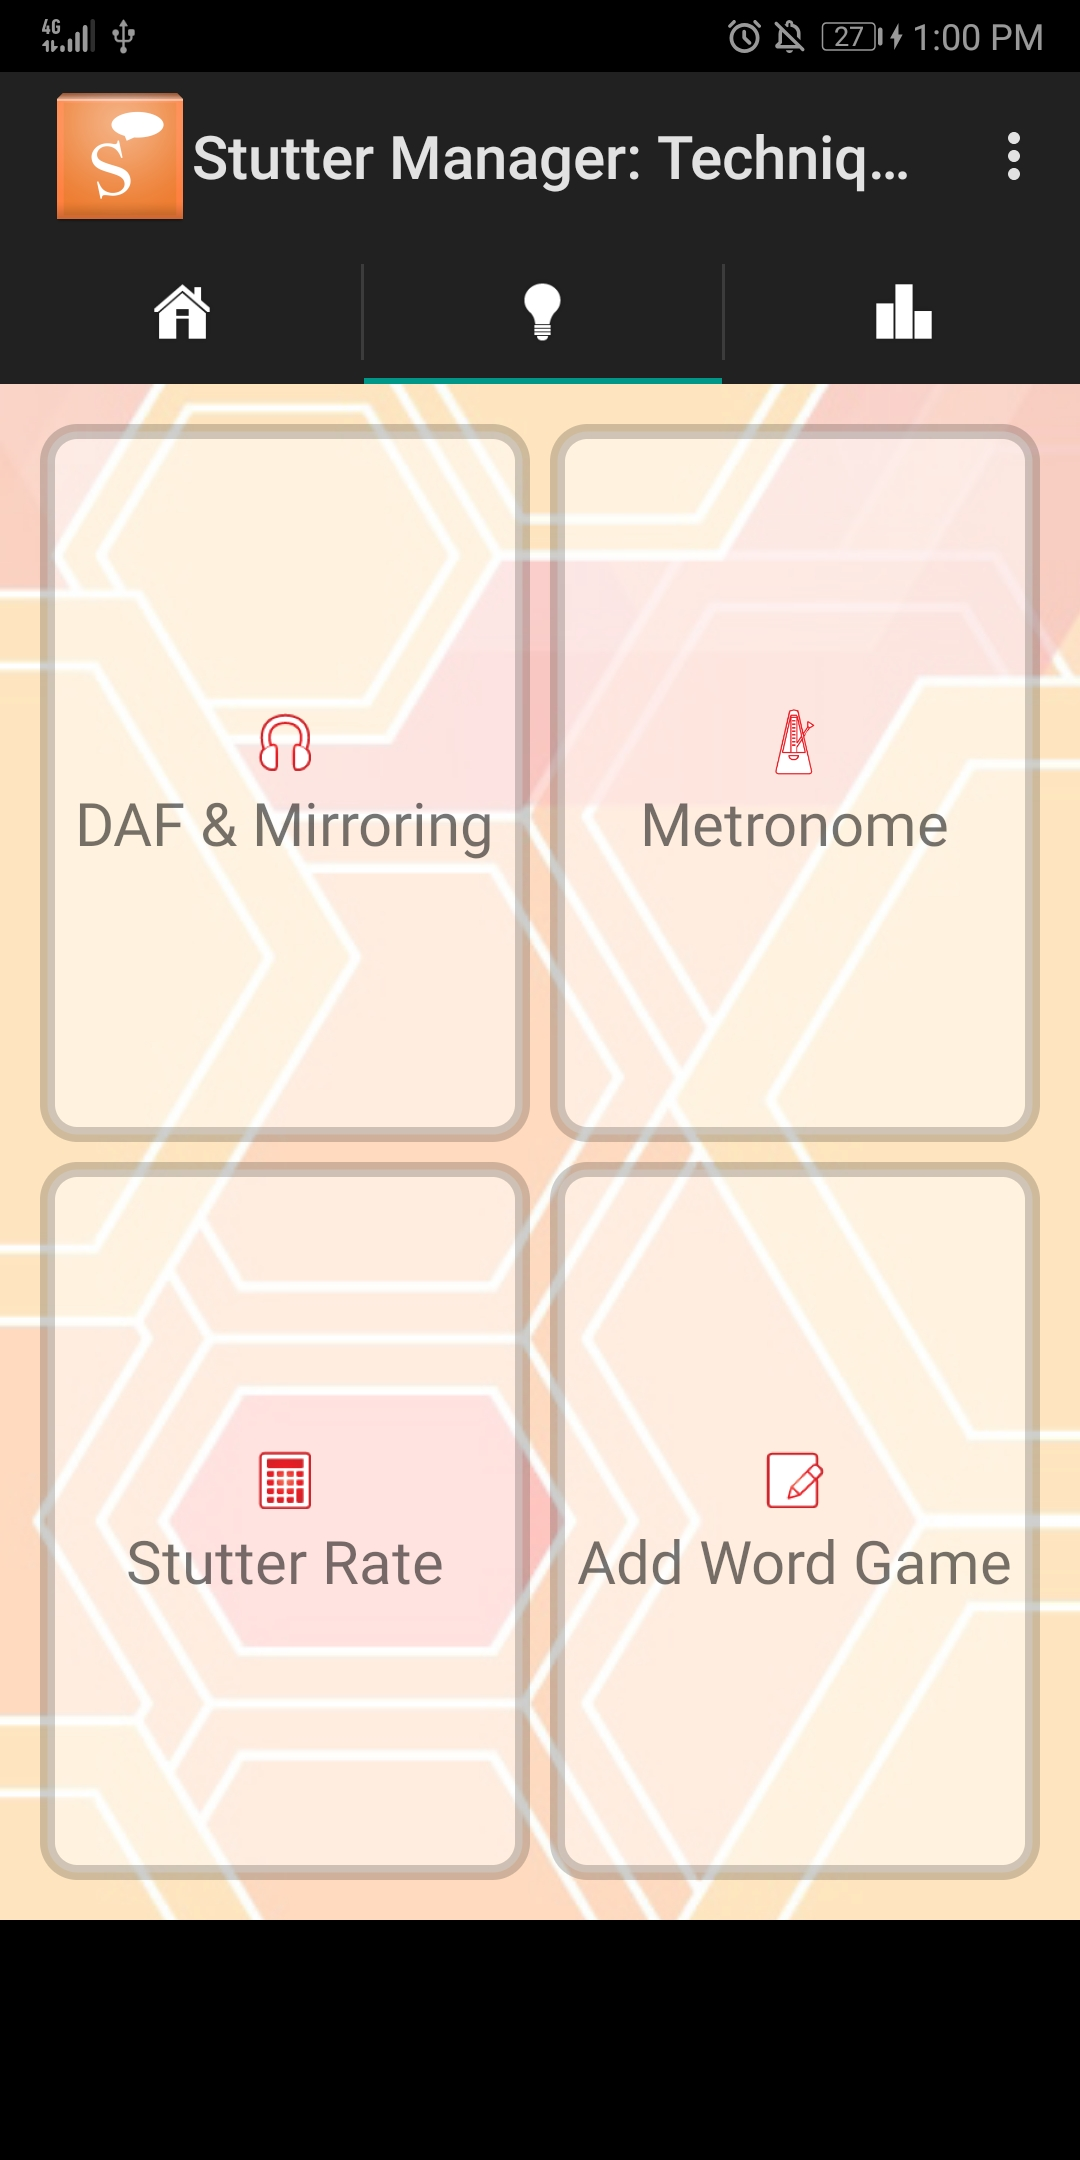
\includegraphics[width=.75\linewidth]{content/imgs/old_app_1.jpg}
    \caption{Page principale (exercices)}
  \end{subfigure}%
  \begin{subfigure}{.25\textwidth}
    \centering
    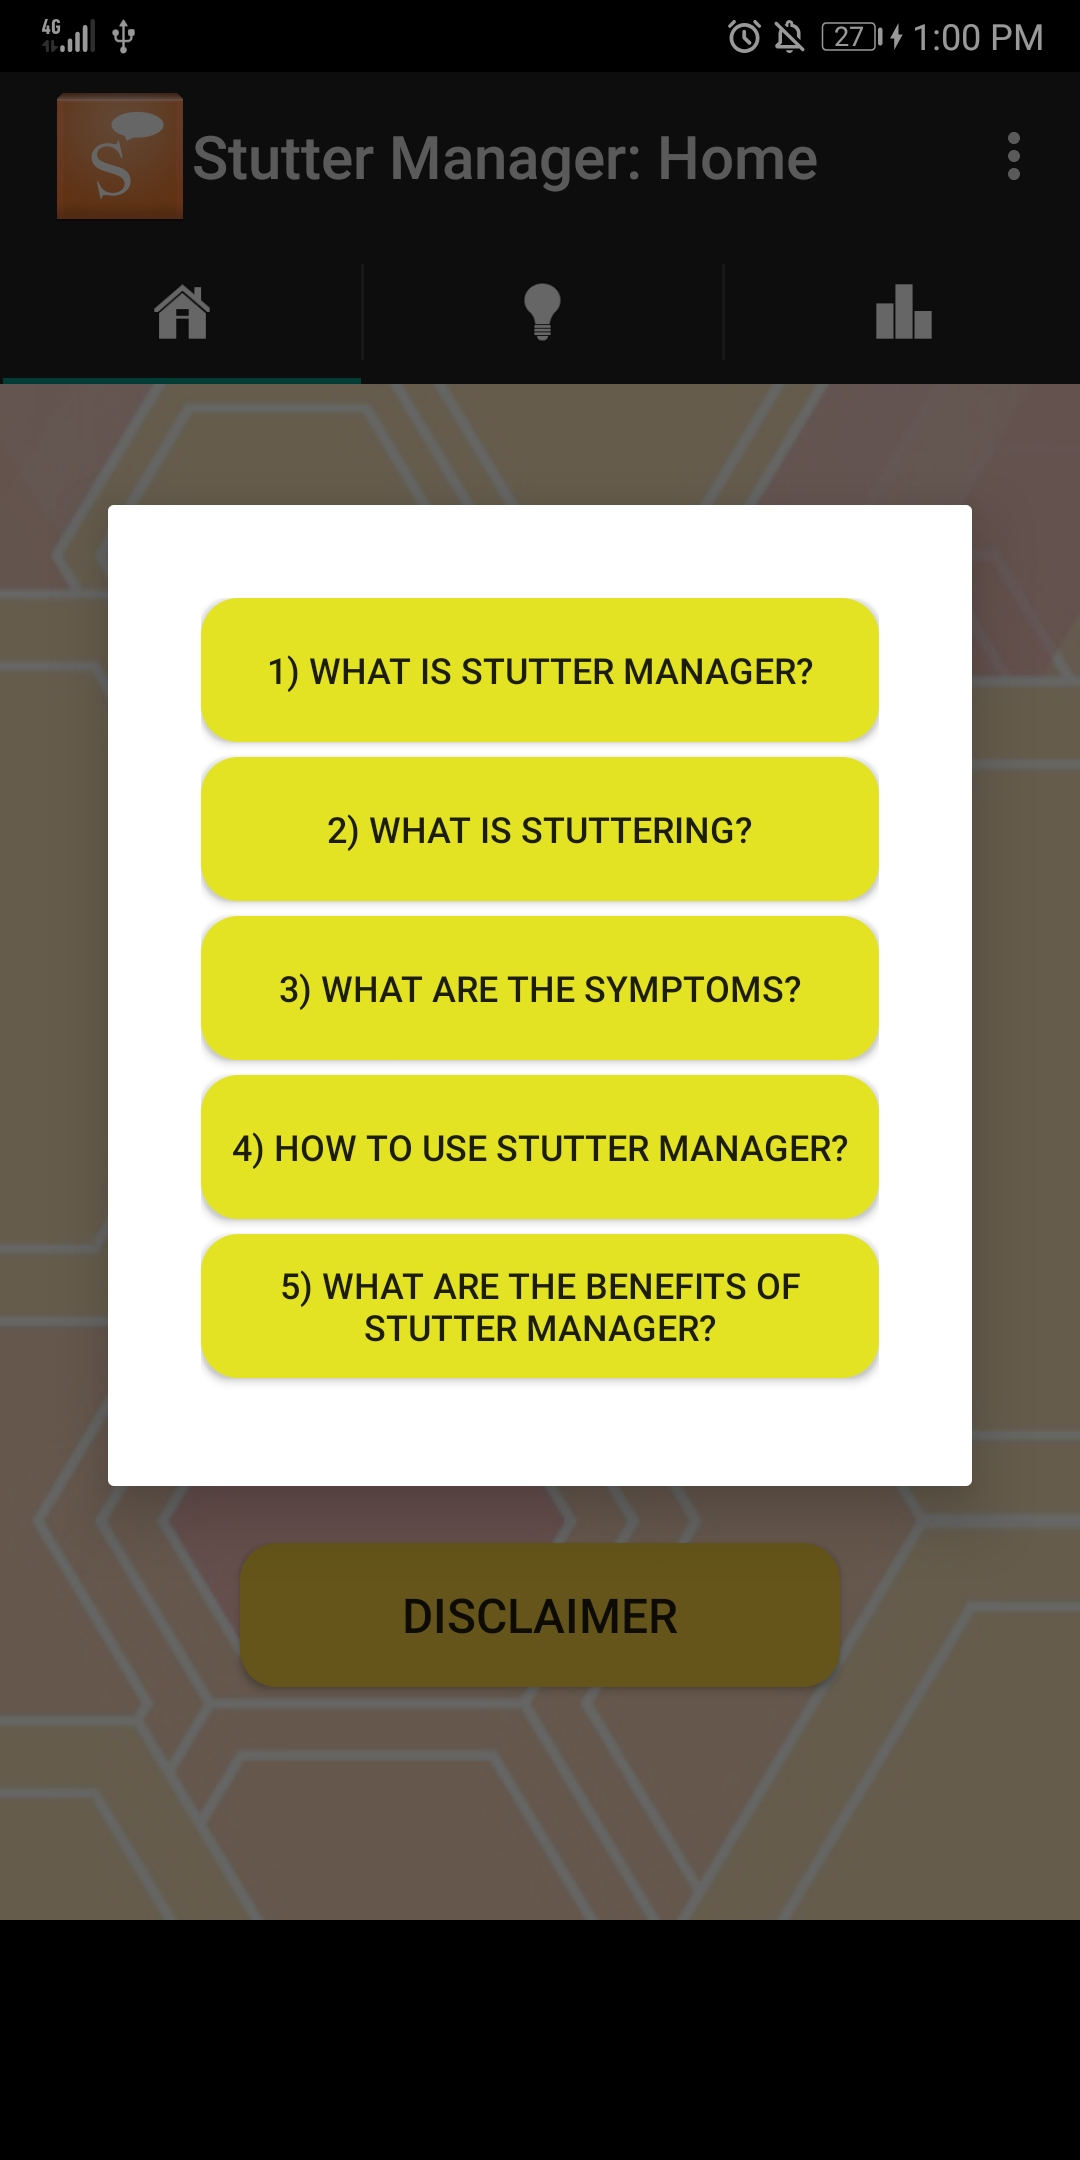
\includegraphics[width=.75\linewidth]{content/imgs/old_app_2.jpg}
    \caption{Informations générales}
  \end{subfigure}%
  \begin{subfigure}{.25\textwidth}
    \centering
    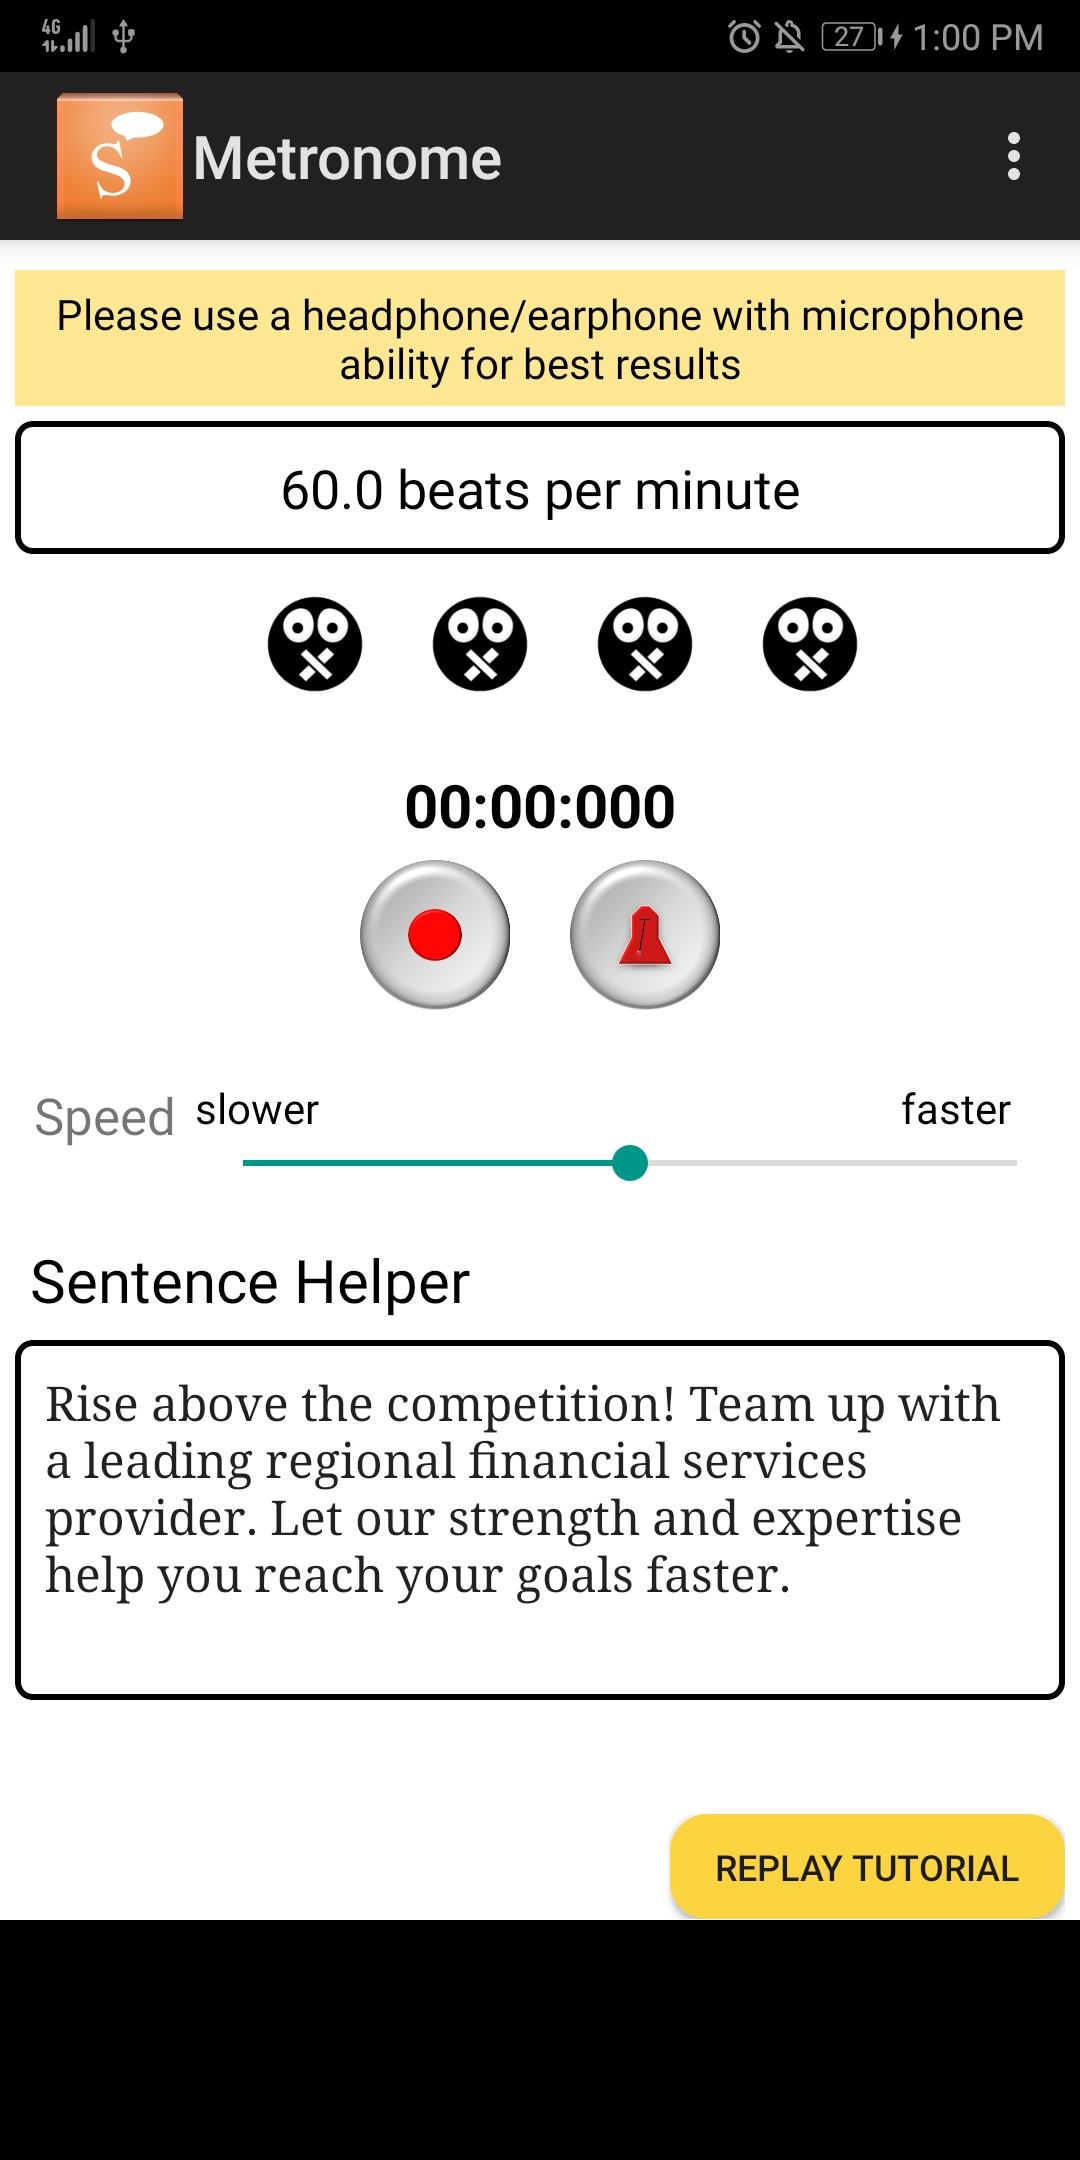
\includegraphics[width=.75\linewidth]{content/imgs/old_app_3.jpg}
    \caption{Exercice : Metronome}
  \end{subfigure}%
  \begin{subfigure}{.25\textwidth}
    \centering
    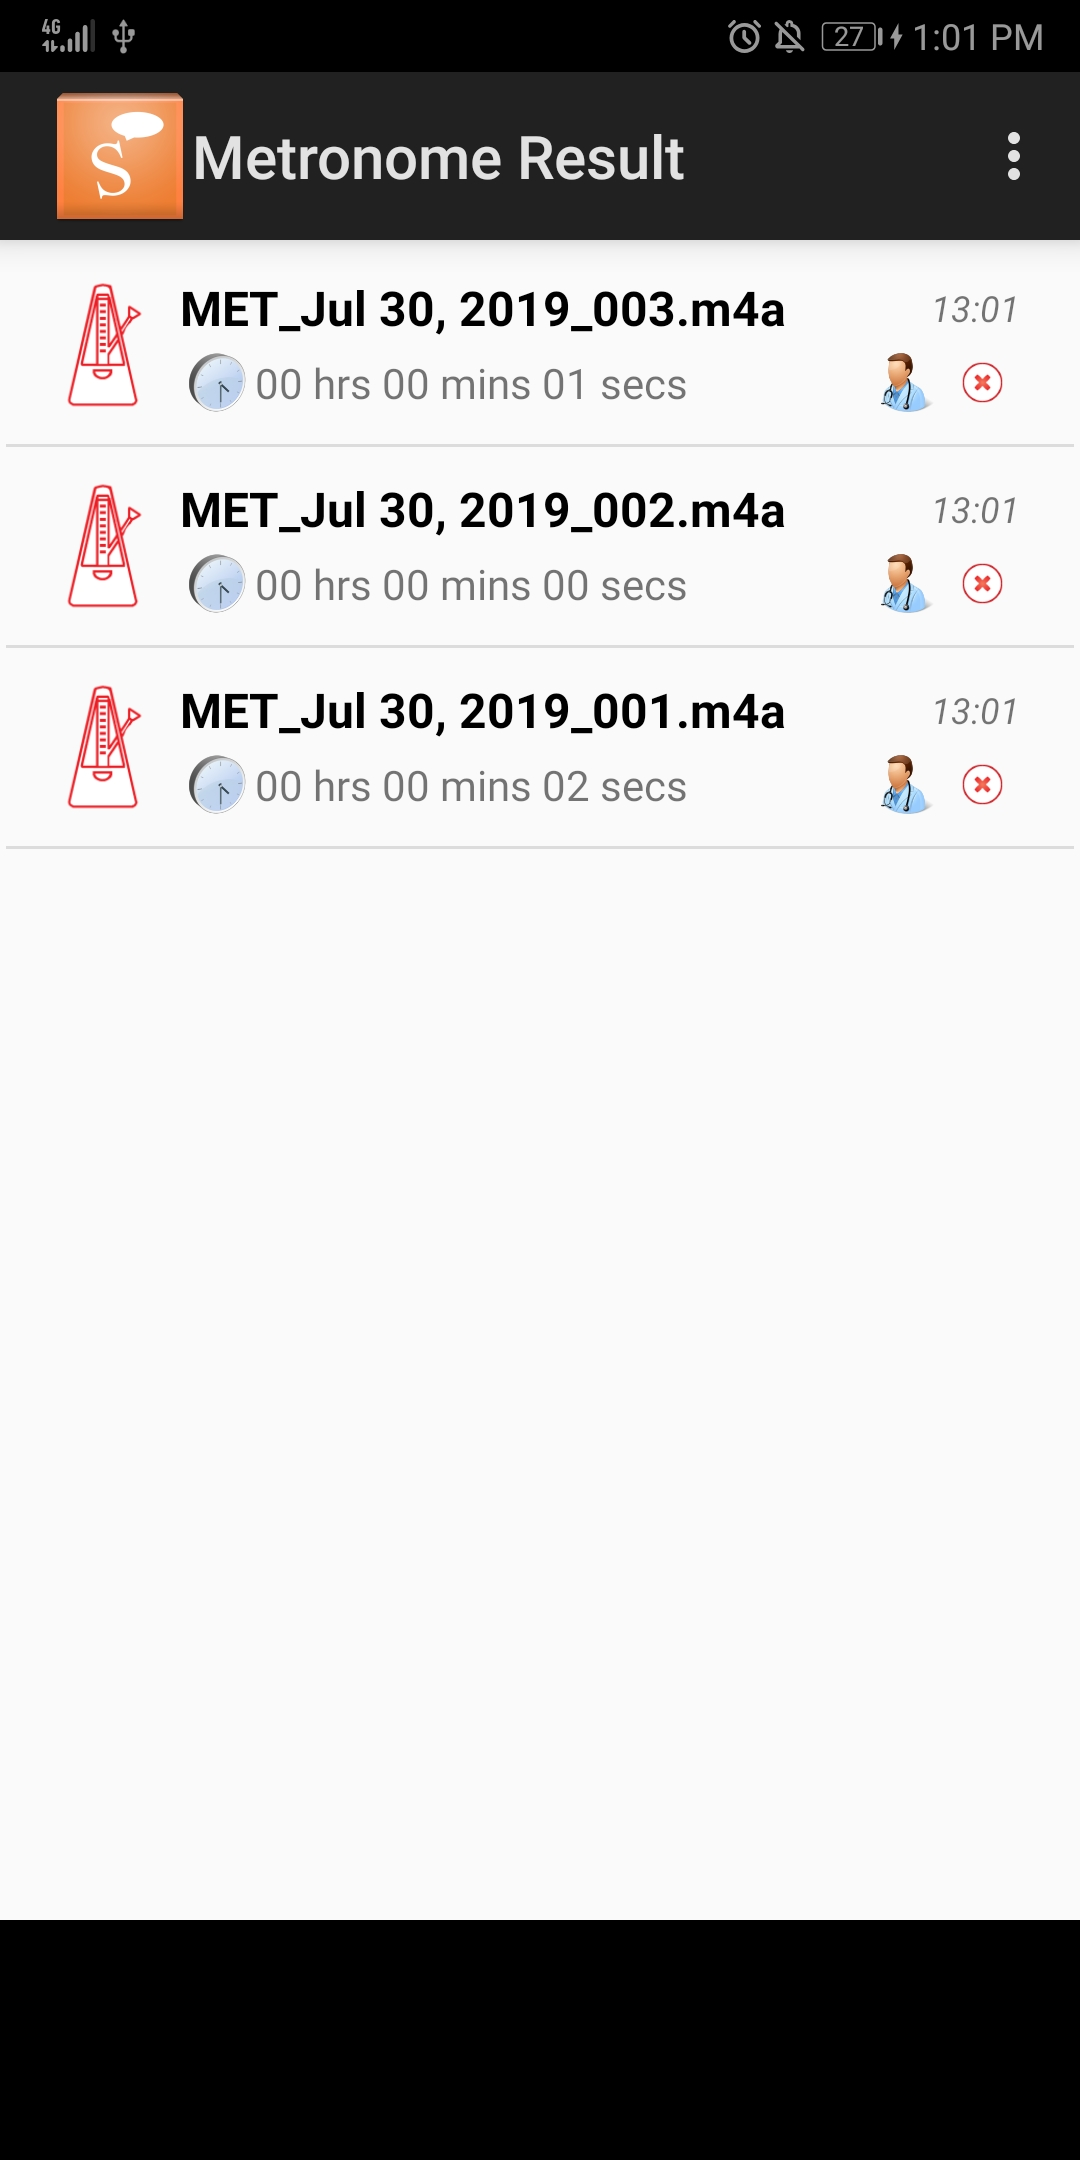
\includegraphics[width=.75\linewidth]{content/imgs/old_app_4.jpg}
    \caption{Progression de l'exercice metronome}
  \end{subfigure}
  \caption*{Captures d'écran de Stutter Manager v3}
\end{figure}

\end{landscape}




\chapter{Étude comparative}
\label{appendix:market}
\begin{figure}[h]
  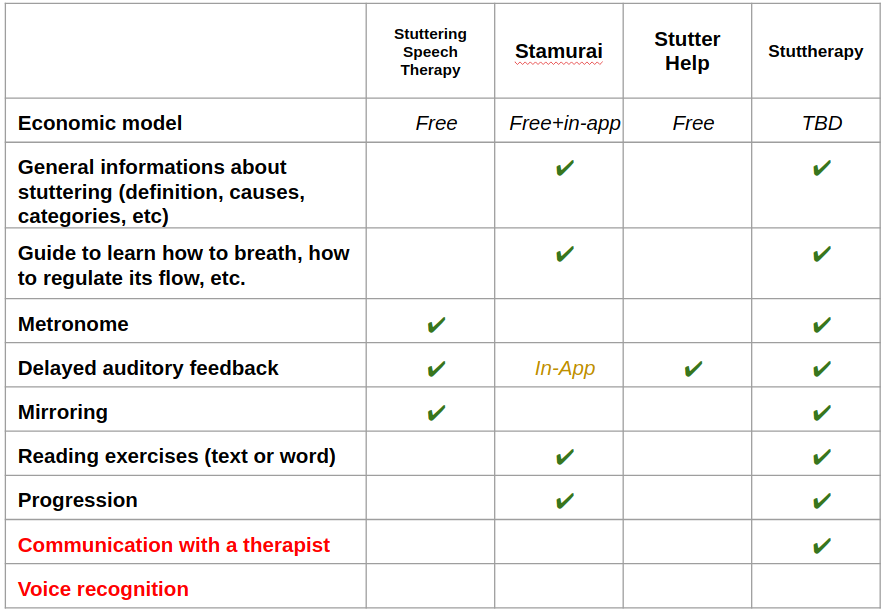
\includegraphics[width=1\linewidth]{content/imgs/market.png}
  \caption*{Étude comparative des applications disponibles sur le Play Store en comparaison avec les fonctionnalités prévues pour Stuttherapy}
\end{figure}



\chapter{Software requirements specification}
\label{appendix:srs}
\begin{figure}[h]
  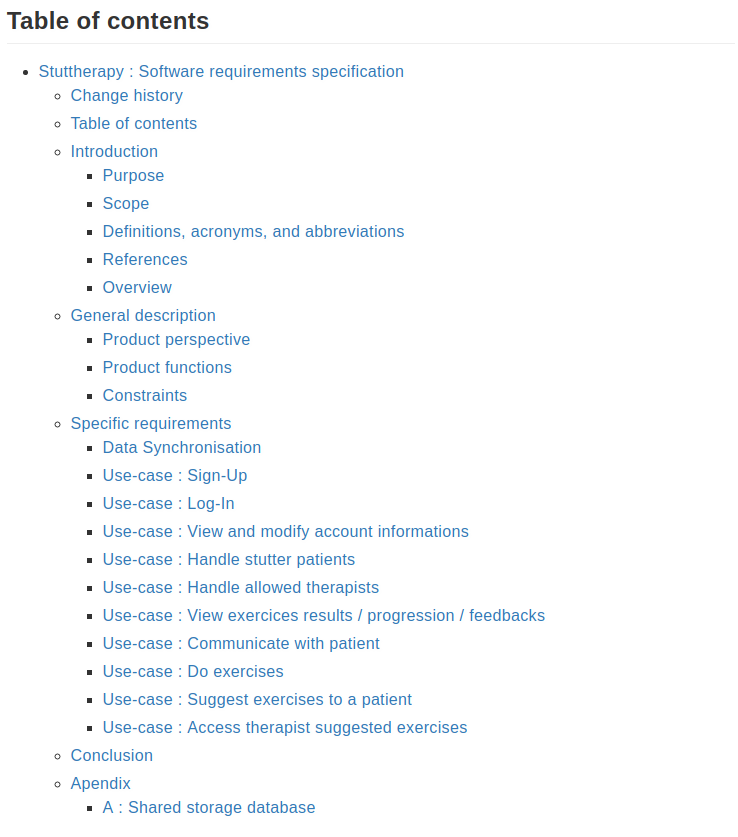
\includegraphics[width=0.7\linewidth]{content/imgs/srs_contents.png}
  \caption*{Table des matières du \textit{Software requirements specification}}
\end{figure}

\begin{displayquote}
The software requirements specification lays out functional and non-functional requirements, and it may include a set of use cases that describe user interactions that the software must provide to the user for perfect interaction.
\end{displayquote}
\hspace*{\fill} \textit{Wikipedia - Software Requirements Specification}


\begin{displayquote}
La spécification des exigences logicielles définit les exigences fonctionnelles et non fonctionnelles. Elle peut inclure un ensemble de cas d'utilisation décrivant les interactions de l'utilisateur que le logiciel doit fournir à l'utilisateur pour obtenir une interaction parfaite.
\end{displayquote}
\hspace*{\fill} \textit{Traduction du passage ci-dessus}


\chapter{Software requirements specifications - Exemple d'un cas d'utilisation}
\label{appendix:srs_example}
\begin{figure}[h]
  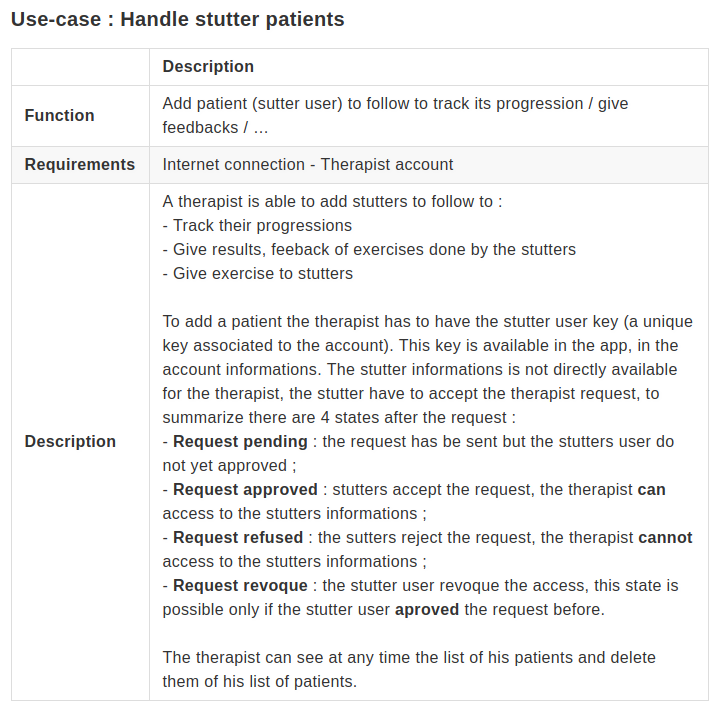
\includegraphics[width=1\linewidth]{content/imgs/srs_use_case_ex.png}
  \caption*{Spécification du cas d'utilisation \textbf{Handle stutter patients}}
\end{figure}




\begin{landscape}
  \label{appendix:gantt}
  \chapter{Diagramme de Gantt prévisionnel}
  \begin{figure}[H]
    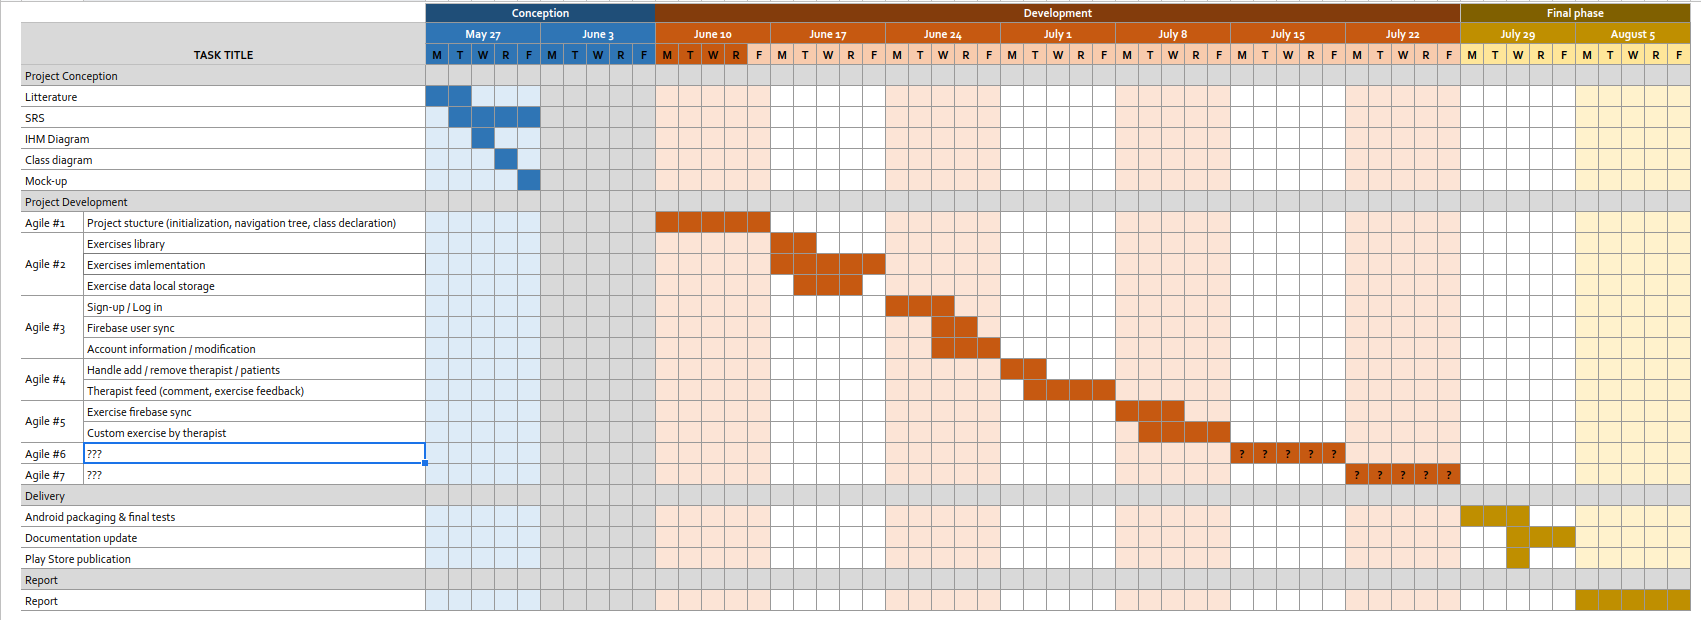
\includegraphics[width=1\linewidth]{content/imgs/gantt.png}
    \caption*{Diagramme de Gantt prévisionnel}
  \end{figure}
\end{landscape}


\chapter{Exemple release Github}
\label{appendix:release}
\begin{figure}[H]
  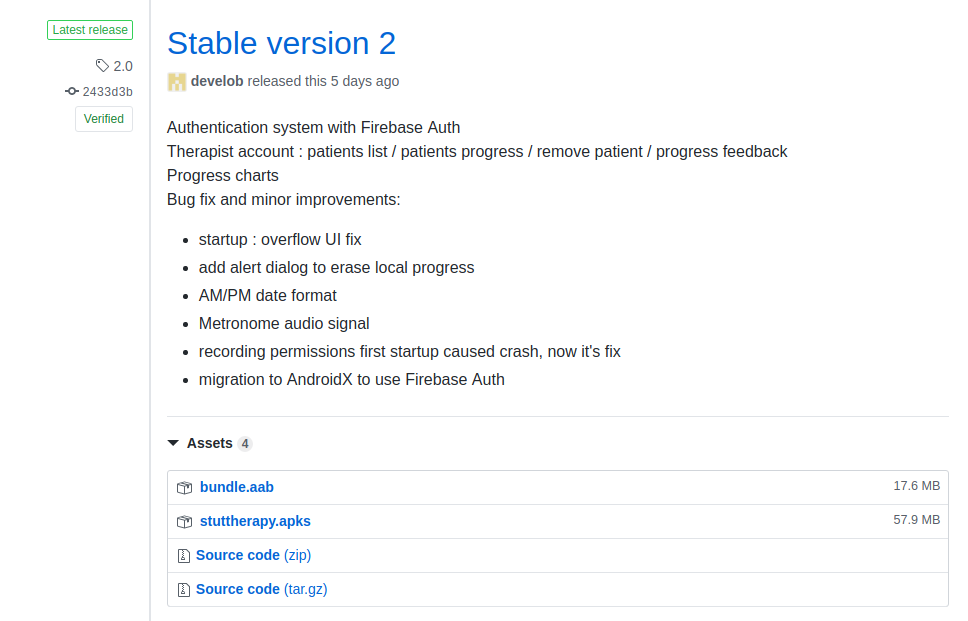
\includegraphics[width=1\linewidth]{content/imgs/release_ex.png}
  \caption*{Release finale de l'application}
\end{figure}

\chapter{Diagramme IHM}
\label{appendix:ihm}
\begin{figure}[H]
  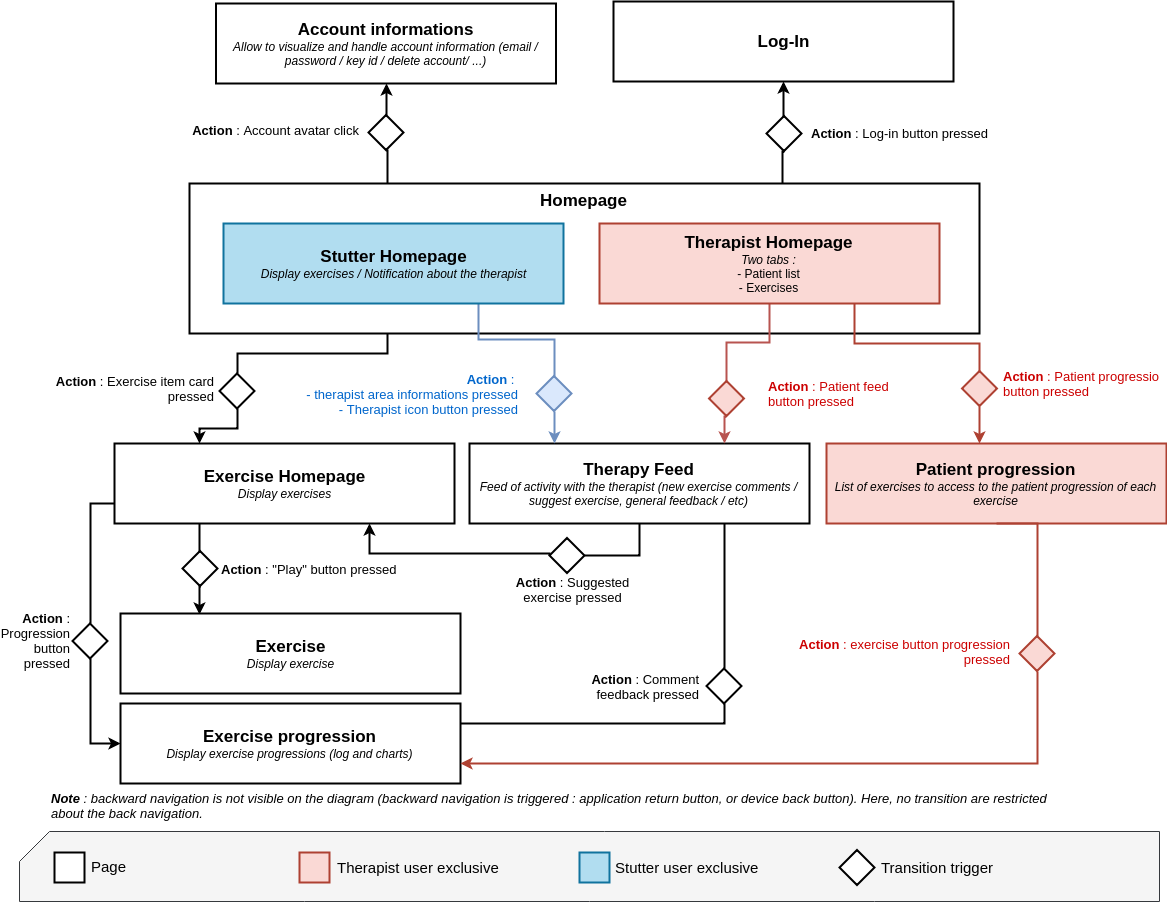
\includegraphics[width=1\linewidth]{content/imgs/IHM_diagram.png}
  \caption*{Diagramme IHM}
\end{figure}


\chapter{Wireframes}
\label{appendix:wireframes}
\section{Pages principales}
\begin{figure}[H]
  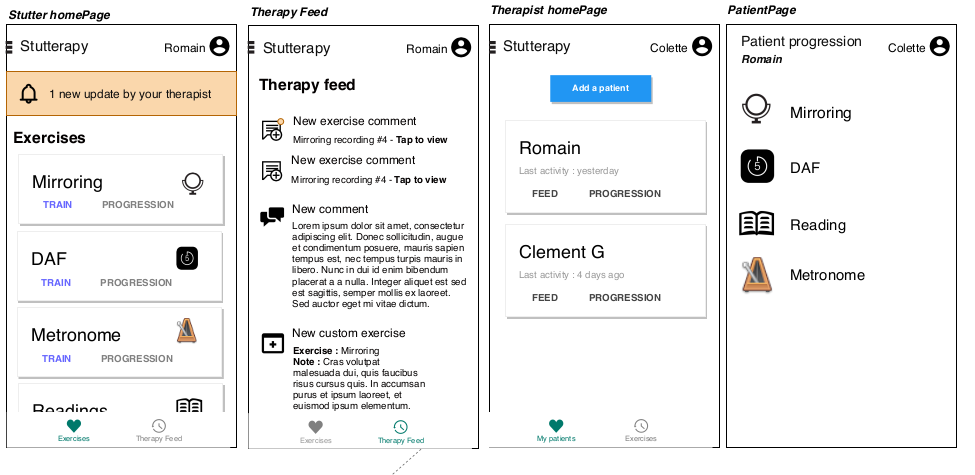
\includegraphics[width=1\linewidth]{content/imgs/maquette1.png}
  \caption*{Pages principales des bègues et des orthopédistes}
\end{figure}

\section{Exercices}
\begin{figure}[H]
  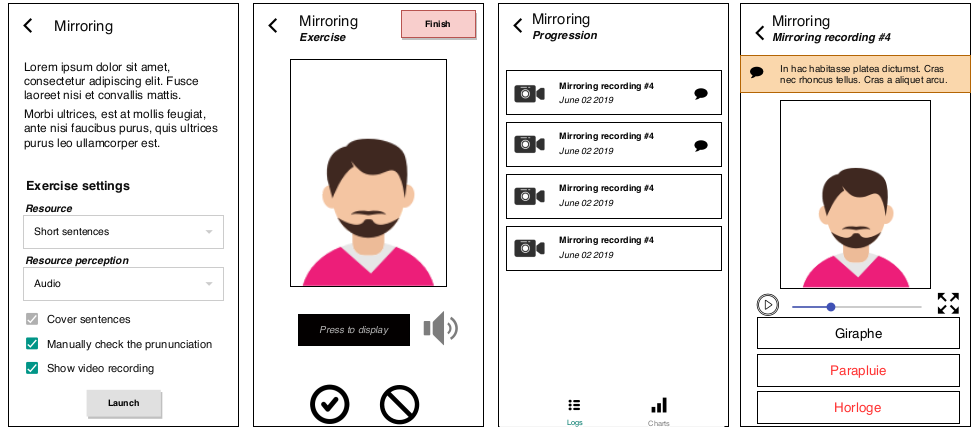
\includegraphics[width=1\linewidth]{content/imgs/maquette2a.png}
  \caption*{Exercice : Mirroring}
\end{figure}

\begin{figure}[H]
  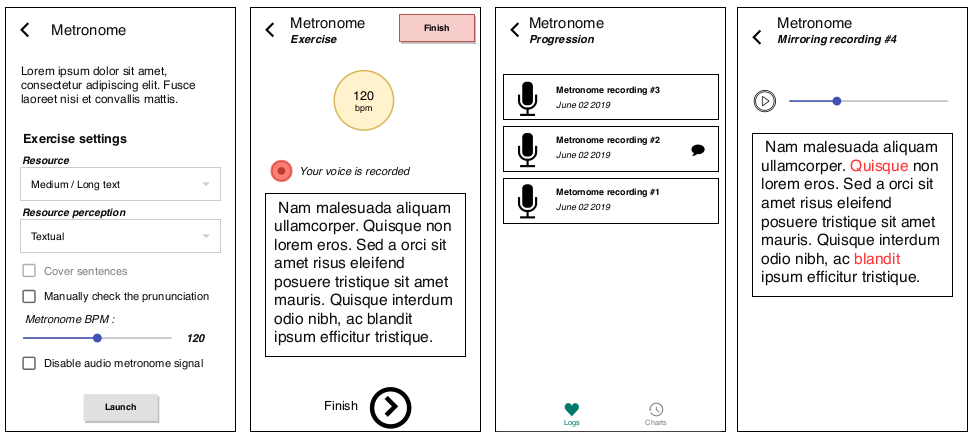
\includegraphics[width=1\linewidth]{content/imgs/maquette2b.png}
  \caption*{Exercice : Metronome}
\end{figure}

\begin{figure}[H]
  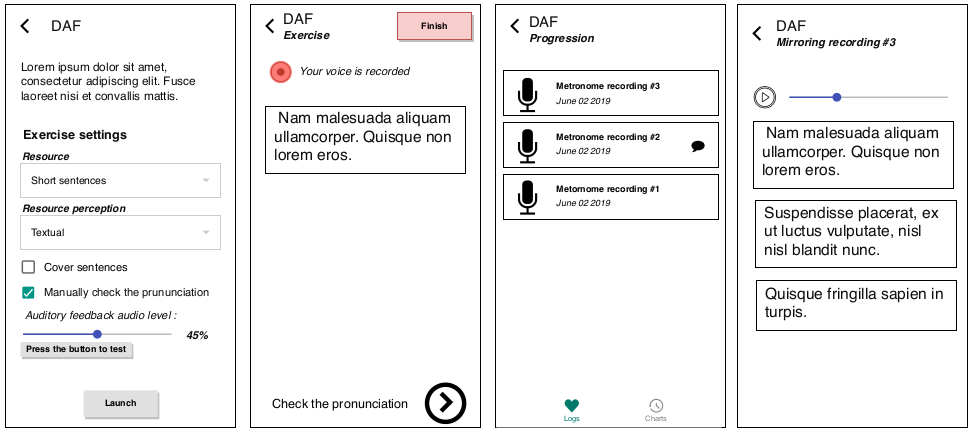
\includegraphics[width=1\linewidth]{content/imgs/maquette2c.png}
  \caption*{Exercice : DAF (delayed auditory feedback)}
\end{figure}

\begin{figure}[H]
  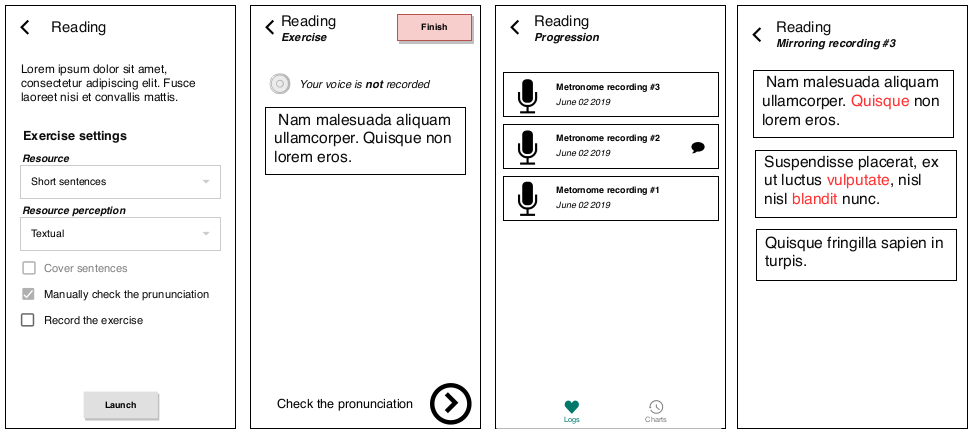
\includegraphics[width=1\linewidth]{content/imgs/maquette2d.png}
  \caption*{Exercice : Reading}
\end{figure}

\section{Divers}
\begin{figure}[H]
  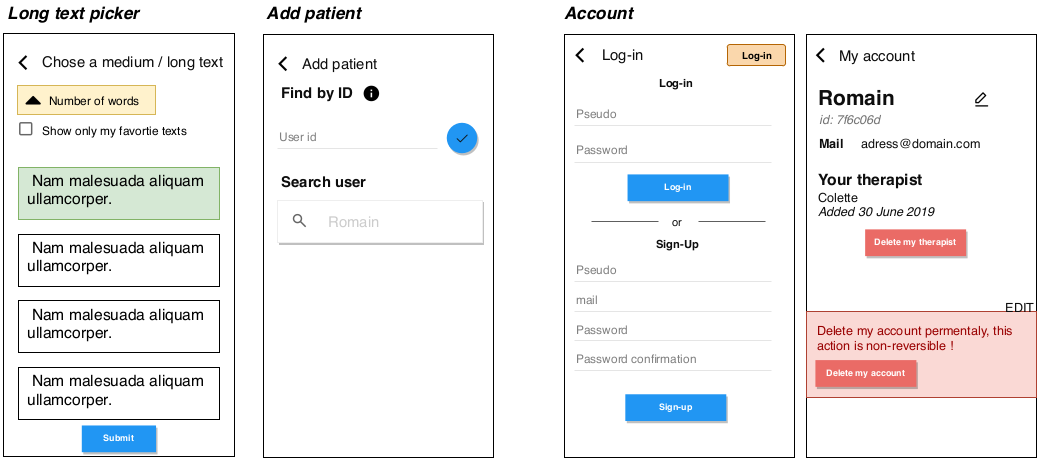
\includegraphics[width=1\linewidth]{content/imgs/maquette3.png}
  \caption*{Sélecteur de textes / ajout d'un patient / informations sur le compte}
\end{figure}






\begin{landscape}
  \chapter{Diagramme de classe}
  \label{appendix:class}
  \vspace{-40pt}
  \begin{figure}[H]
    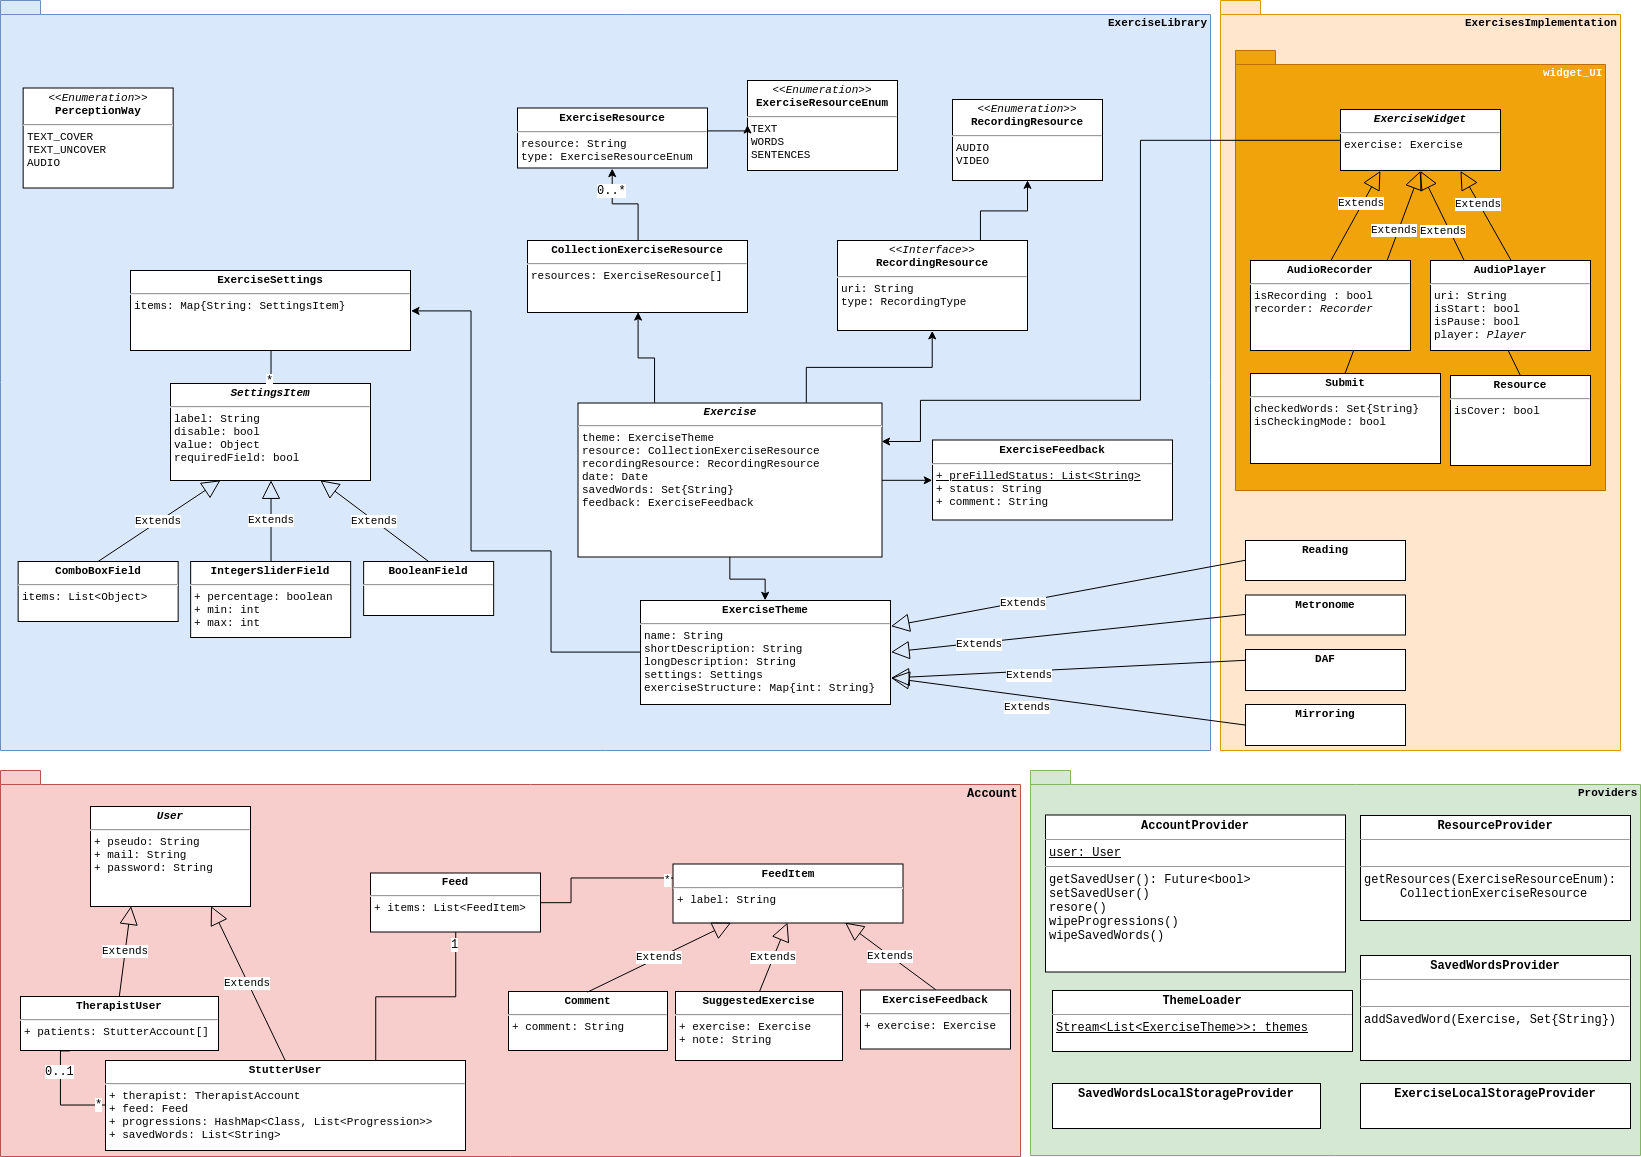
\includegraphics[width=1\linewidth]{content/imgs/app_class_diagram.png}
    % \caption*{Diagramme IHM}
  \end{figure}
\end{landscape}


\begin{landscape}
\chapter{Stuttherapy - Captures d'écran}
\label{appendix:screenshots}

\begin{figure}[h]
  \centering
  \begin{subfigure}{.25\textwidth}
    \centering
    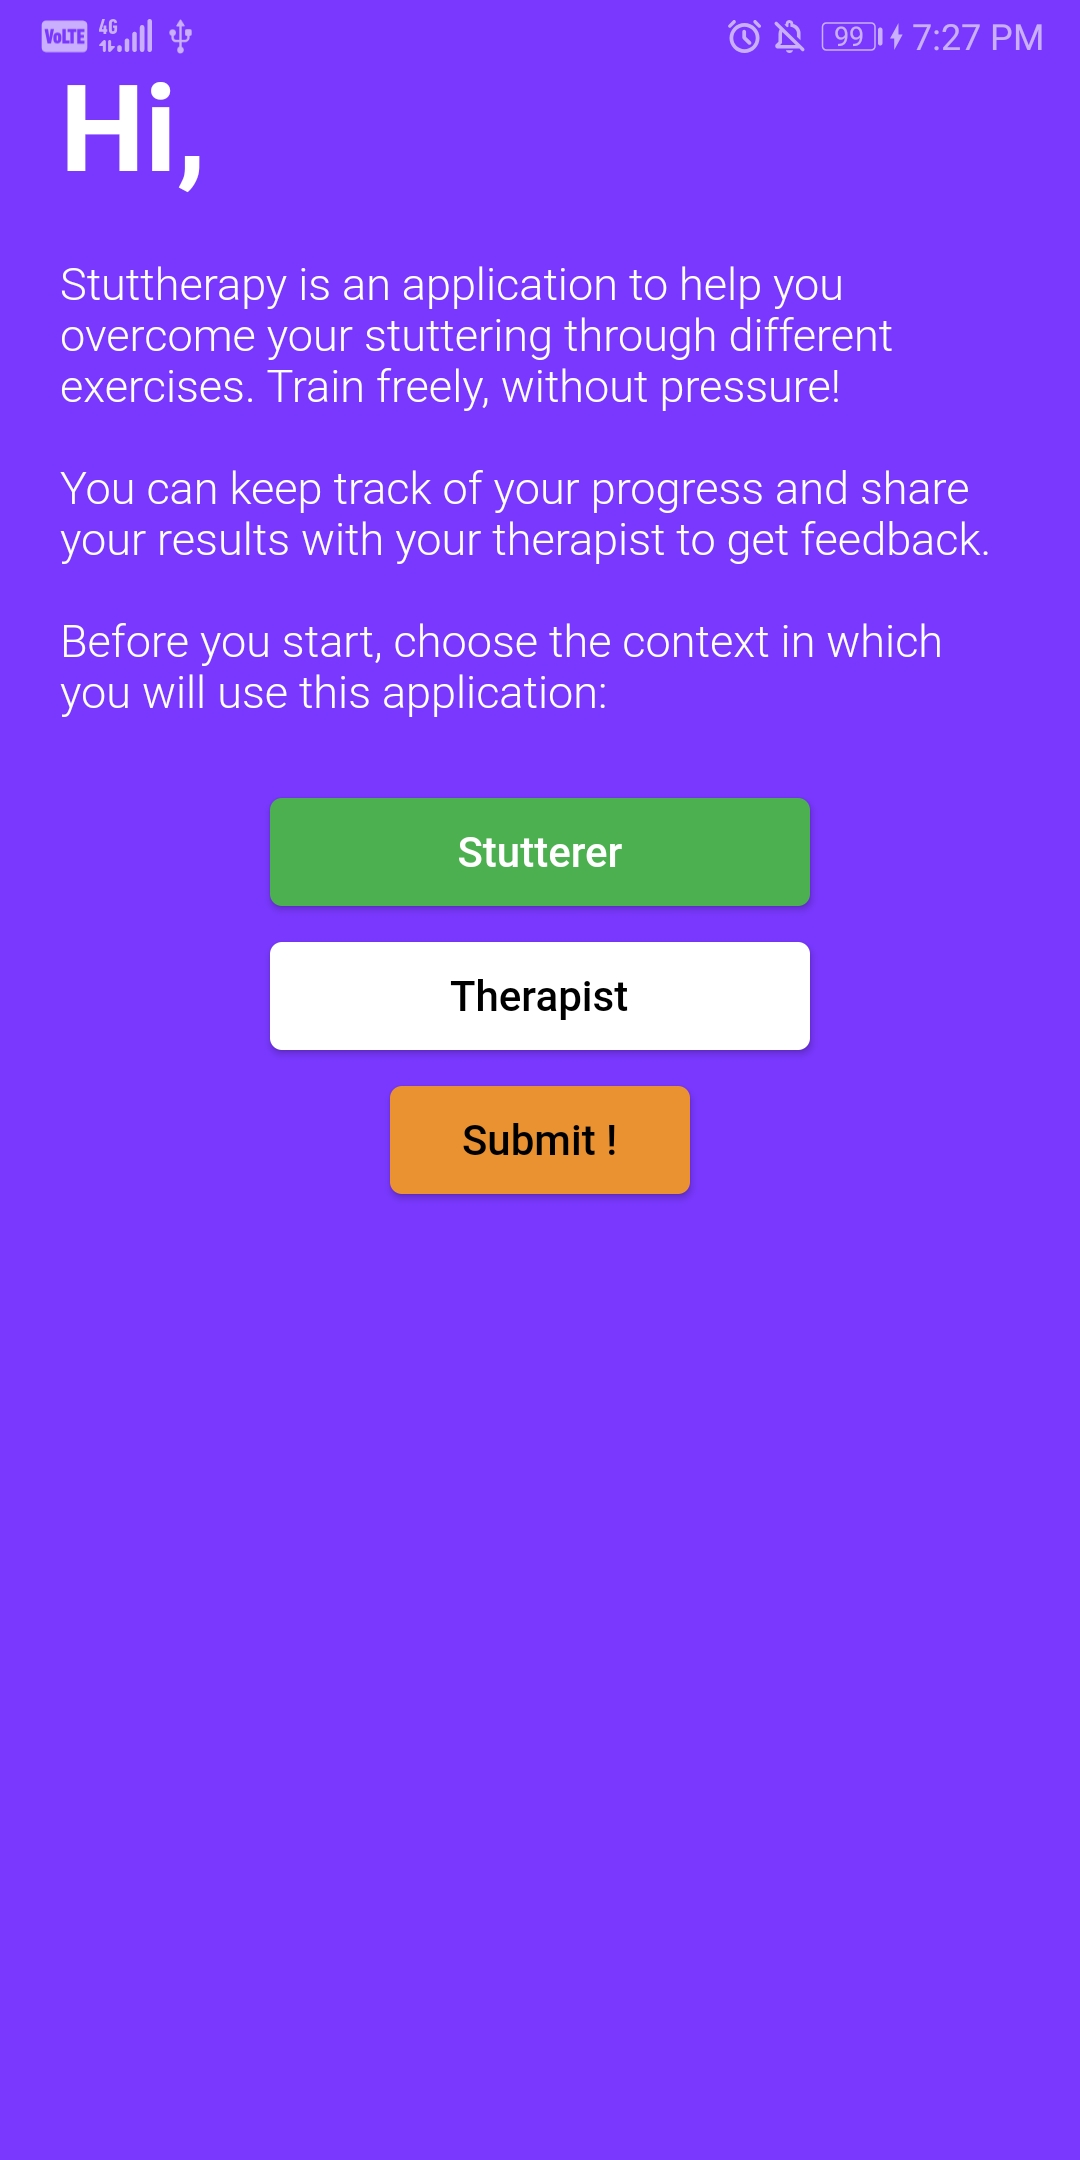
\includegraphics[width=.75\linewidth]{content/imgs/screen1.jpg}
    \caption{Page lors du premier démarrage}
    \label{appendix:screen_start}
  \end{subfigure}%
  \begin{subfigure}{.25\textwidth}
    \centering
    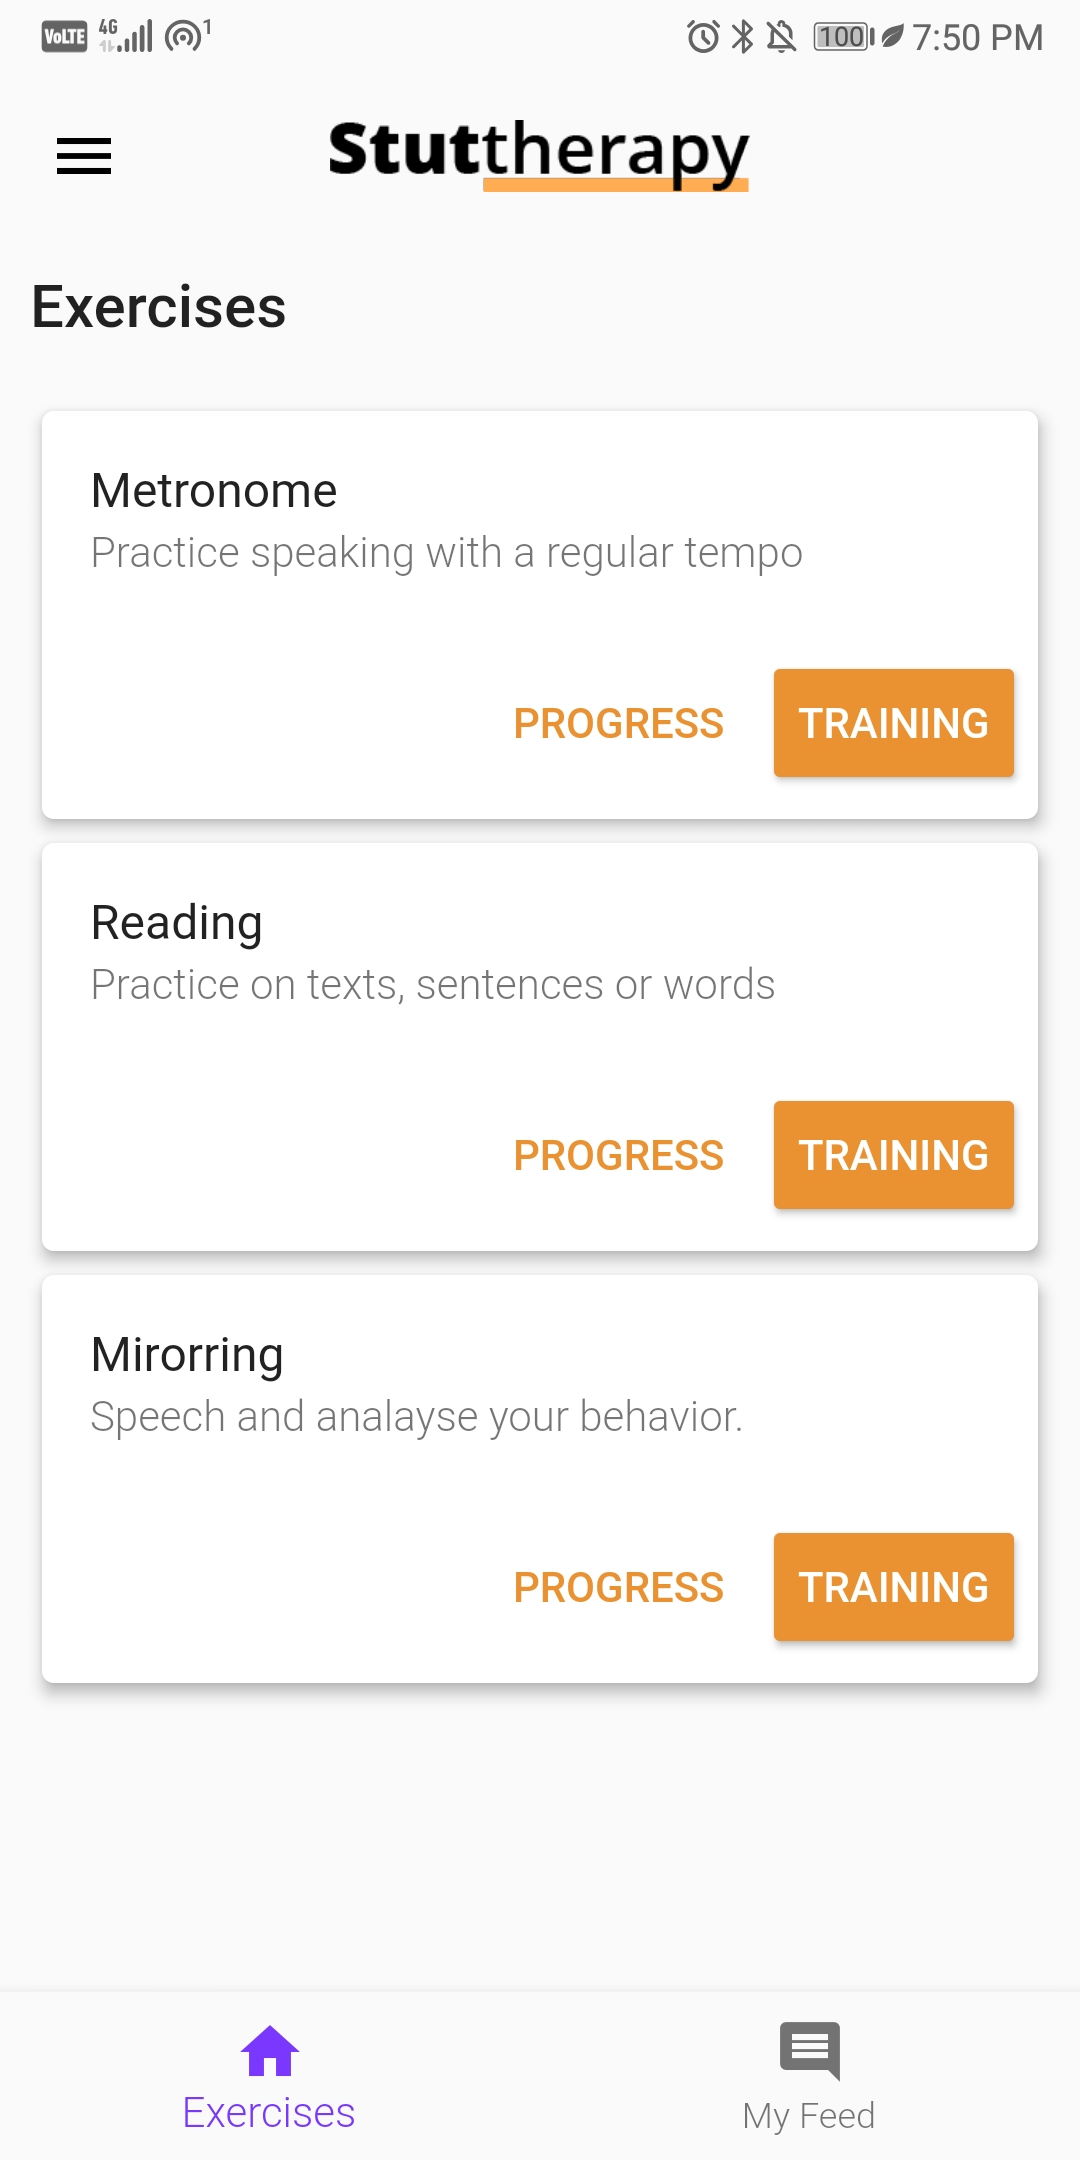
\includegraphics[width=.75\linewidth]{content/imgs/screen2.jpg}
    \caption{Liste des exercices disponibles}
    \label{appendix:screen_exercises}
  \end{subfigure}%
  \begin{subfigure}{.25\textwidth}
    \centering
    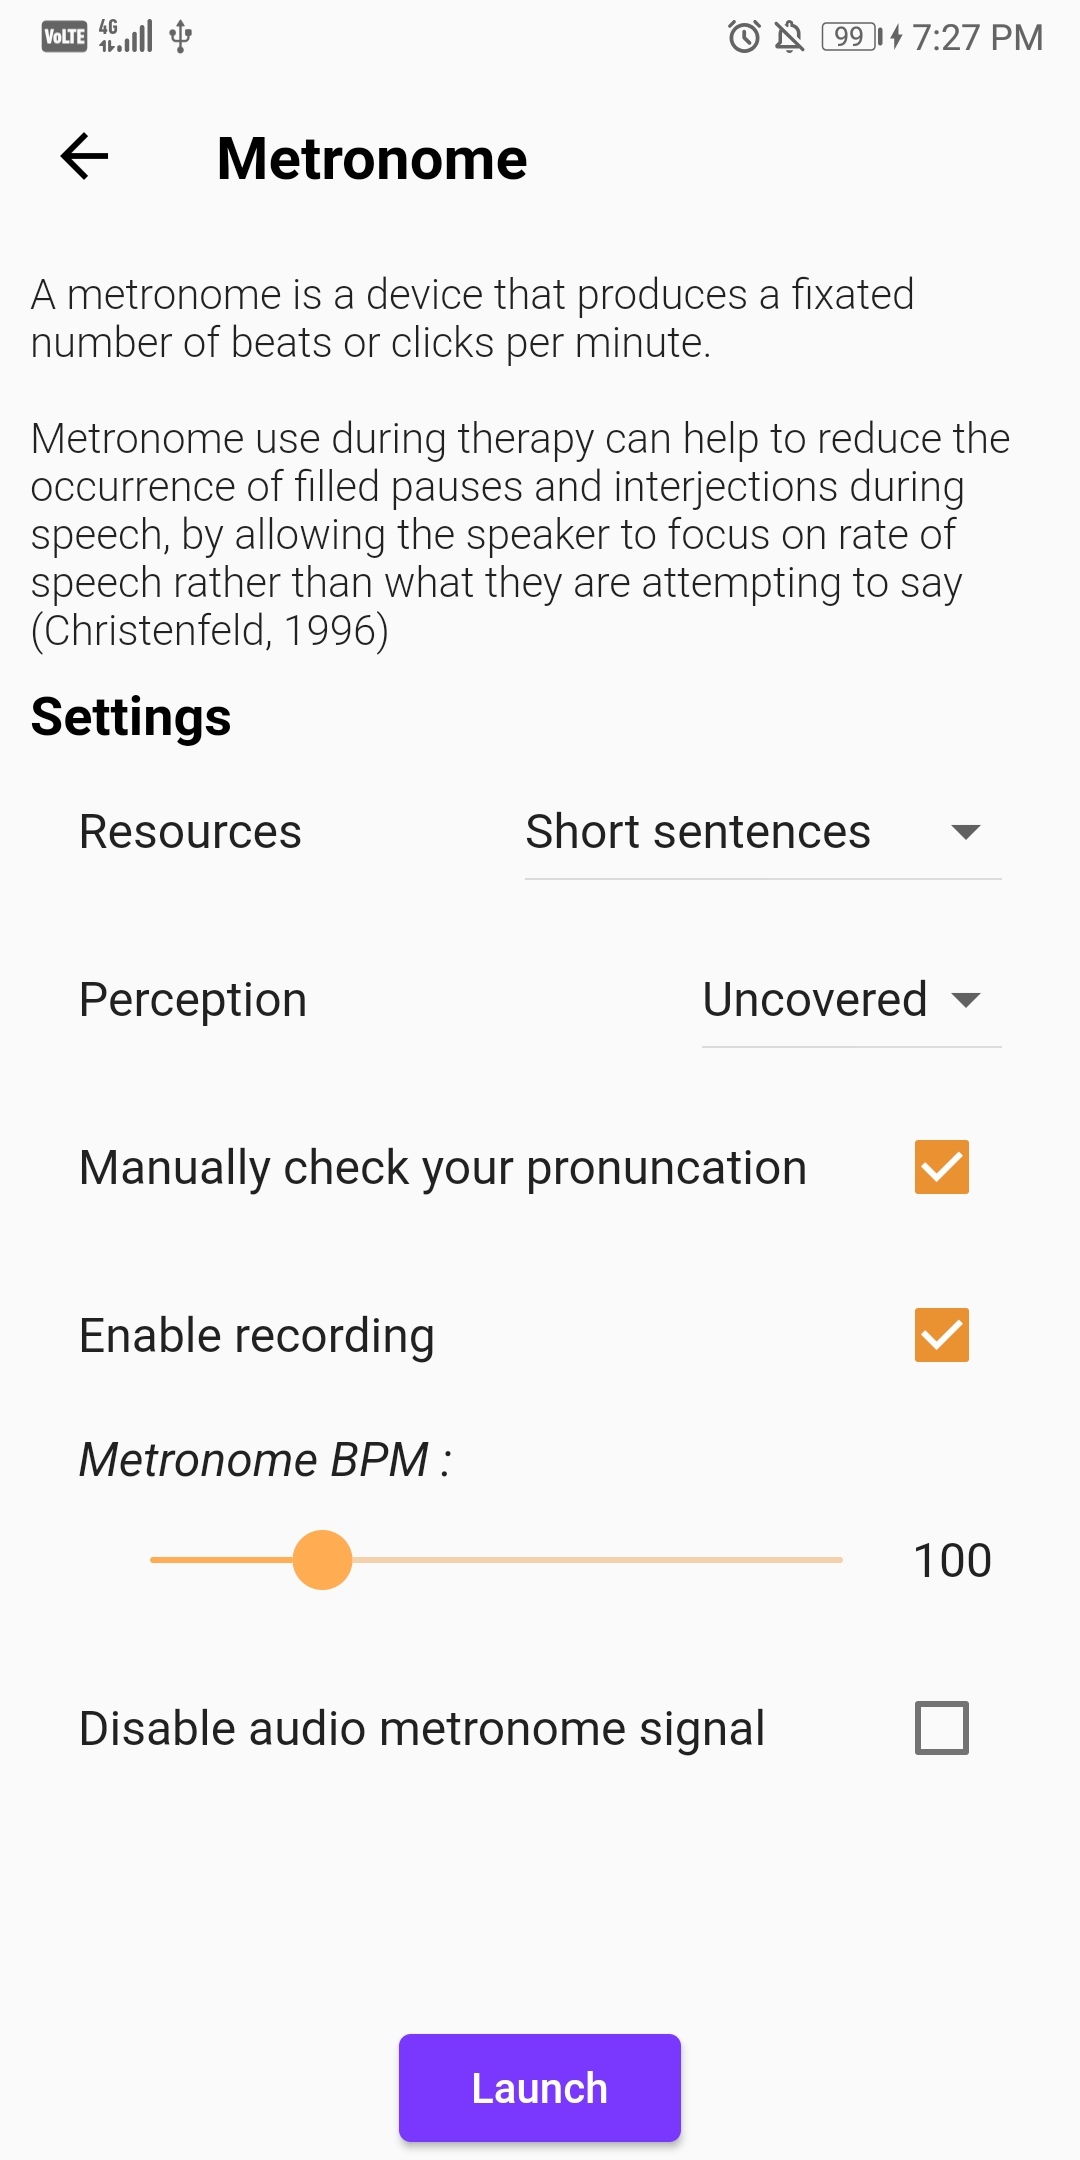
\includegraphics[width=.75\linewidth]{content/imgs/screen3.jpg}
    \caption{Page d'accueil de l'exercice \textit{metronome}}
    \label{appendix:screen_metronome}
  \end{subfigure}%
  \begin{subfigure}{.25\textwidth}
    \centering
    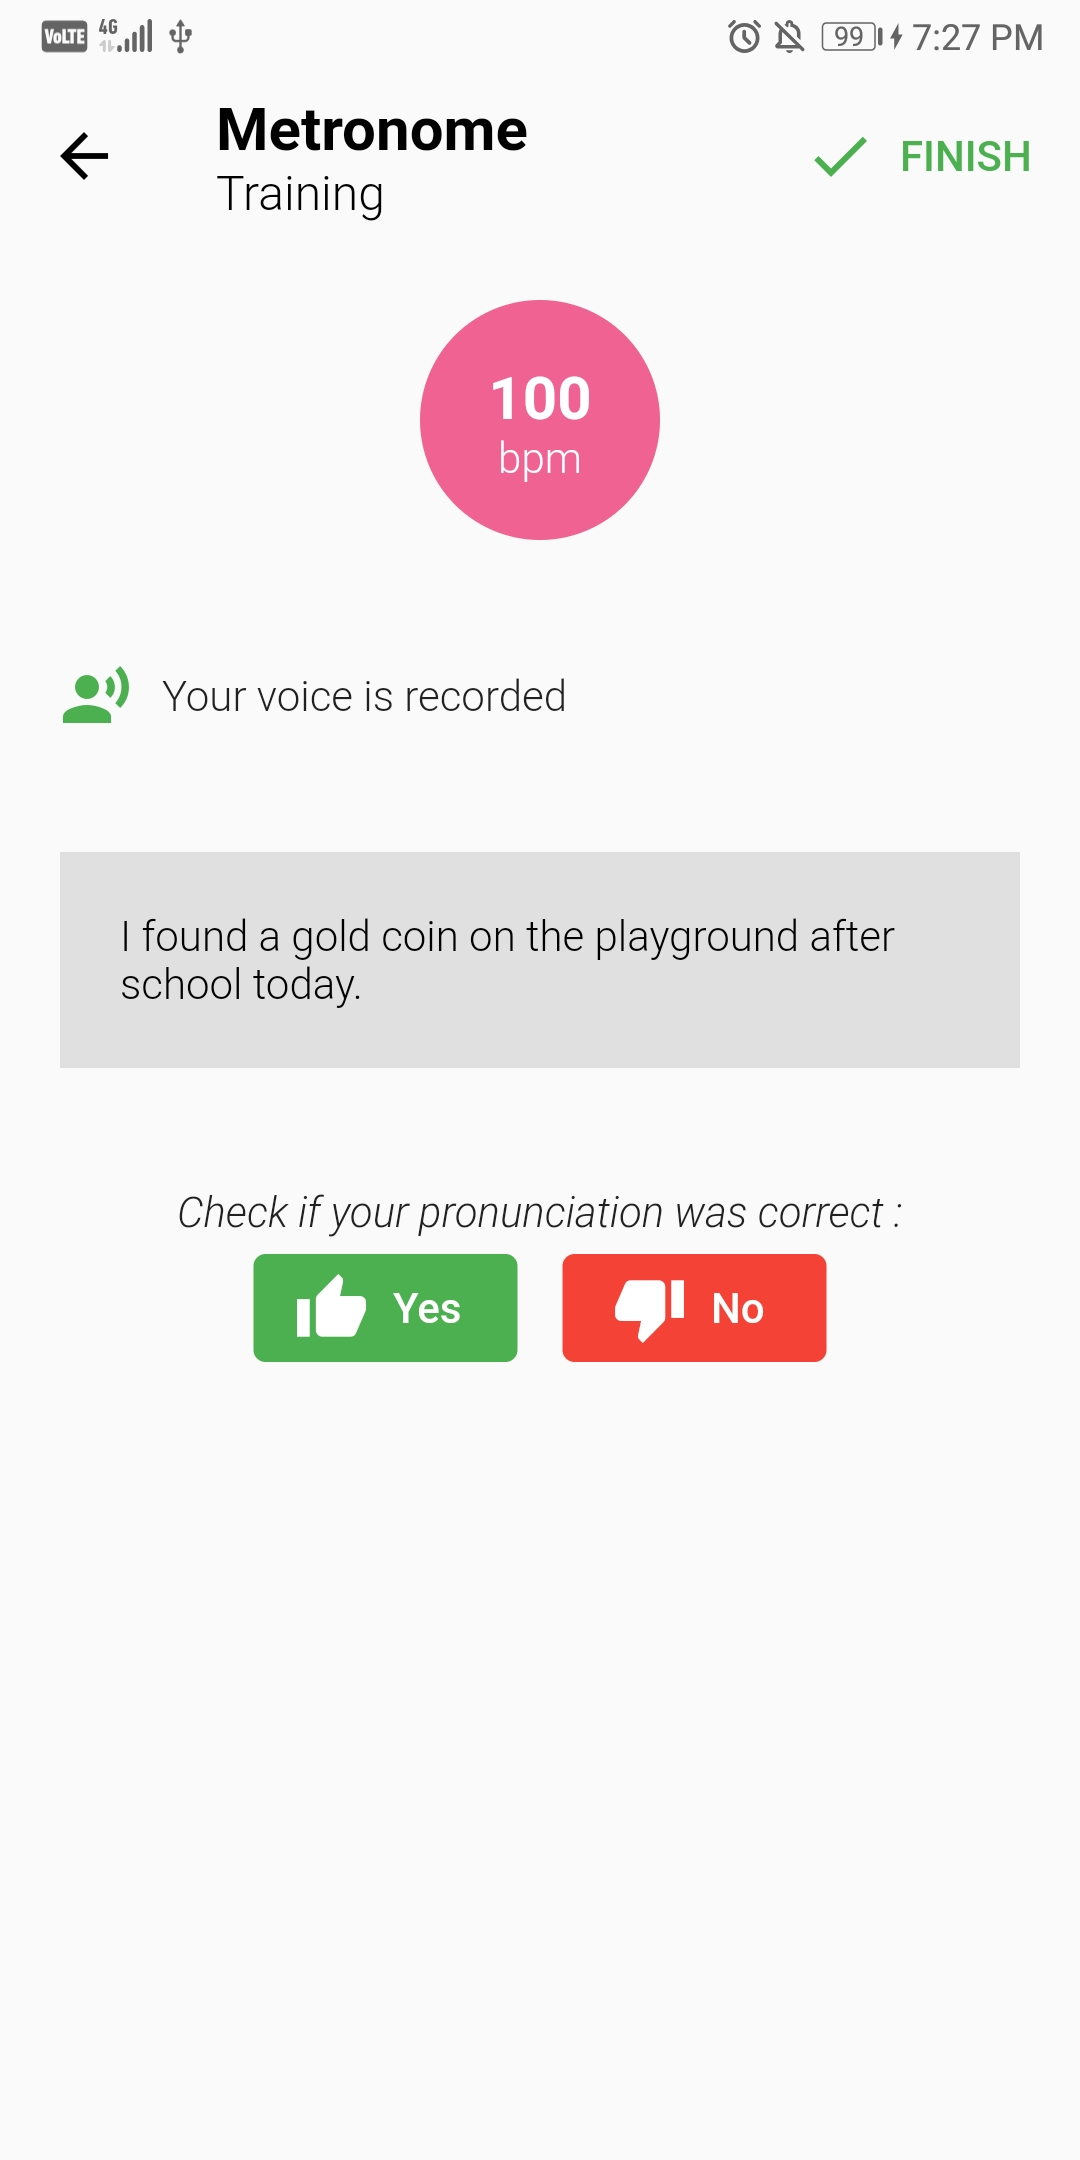
\includegraphics[width=.75\linewidth]{content/imgs/screen4.jpg}
    \caption{Entraînement sur l'exercice \textit{metronome}}
    \label{appendix:screen_metronome_train}
  \end{subfigure}
\end{figure}


\begin{figure}[h]
  \begin{subfigure}{.25\textwidth}
    \centering
    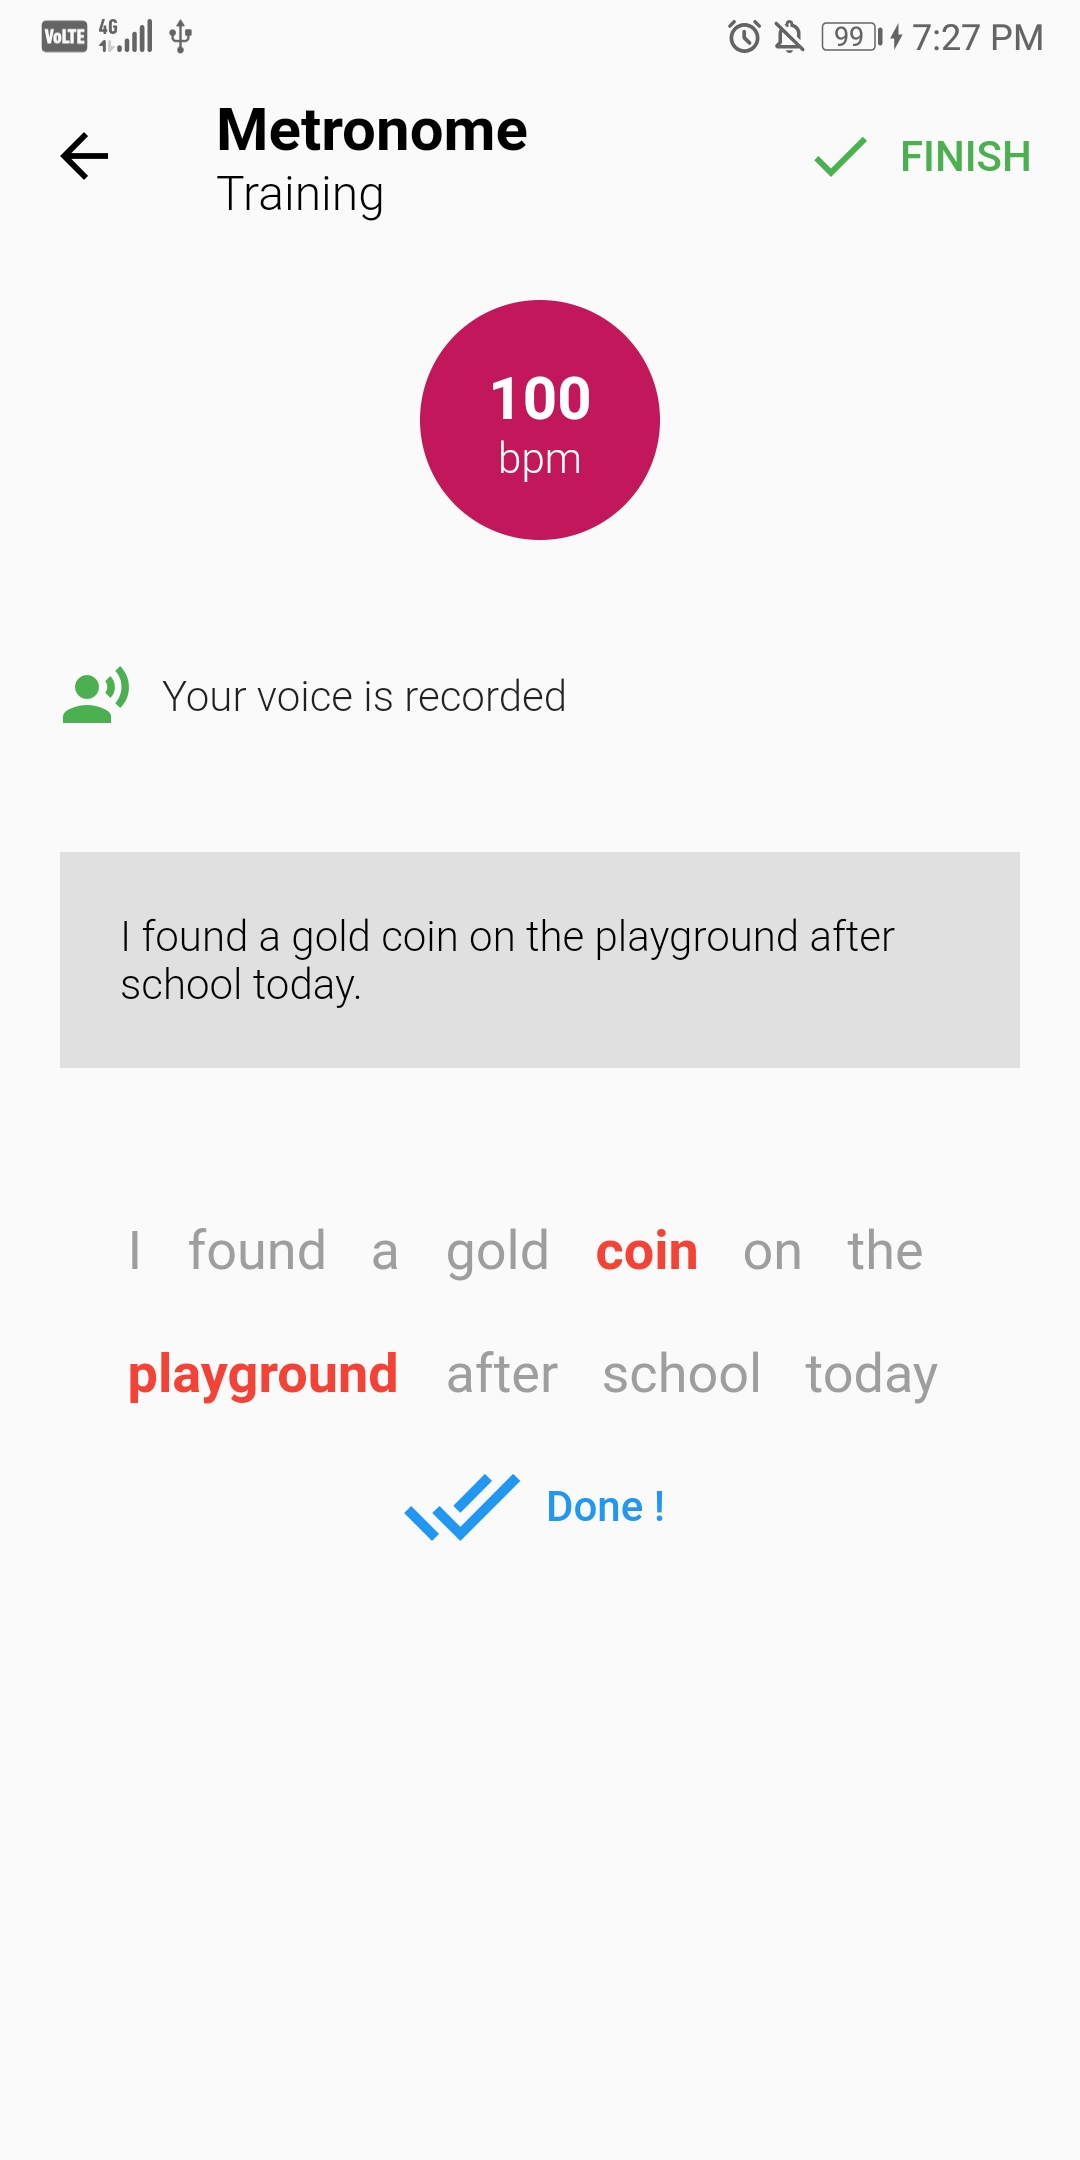
\includegraphics[width=.75\linewidth]{content/imgs/screen5.jpg}
    \caption{Selection des mots mal prononcés}
    \label{appendix:screen_exercice_words_check}
  \end{subfigure}%
  \begin{subfigure}{.25\textwidth}
    \centering
    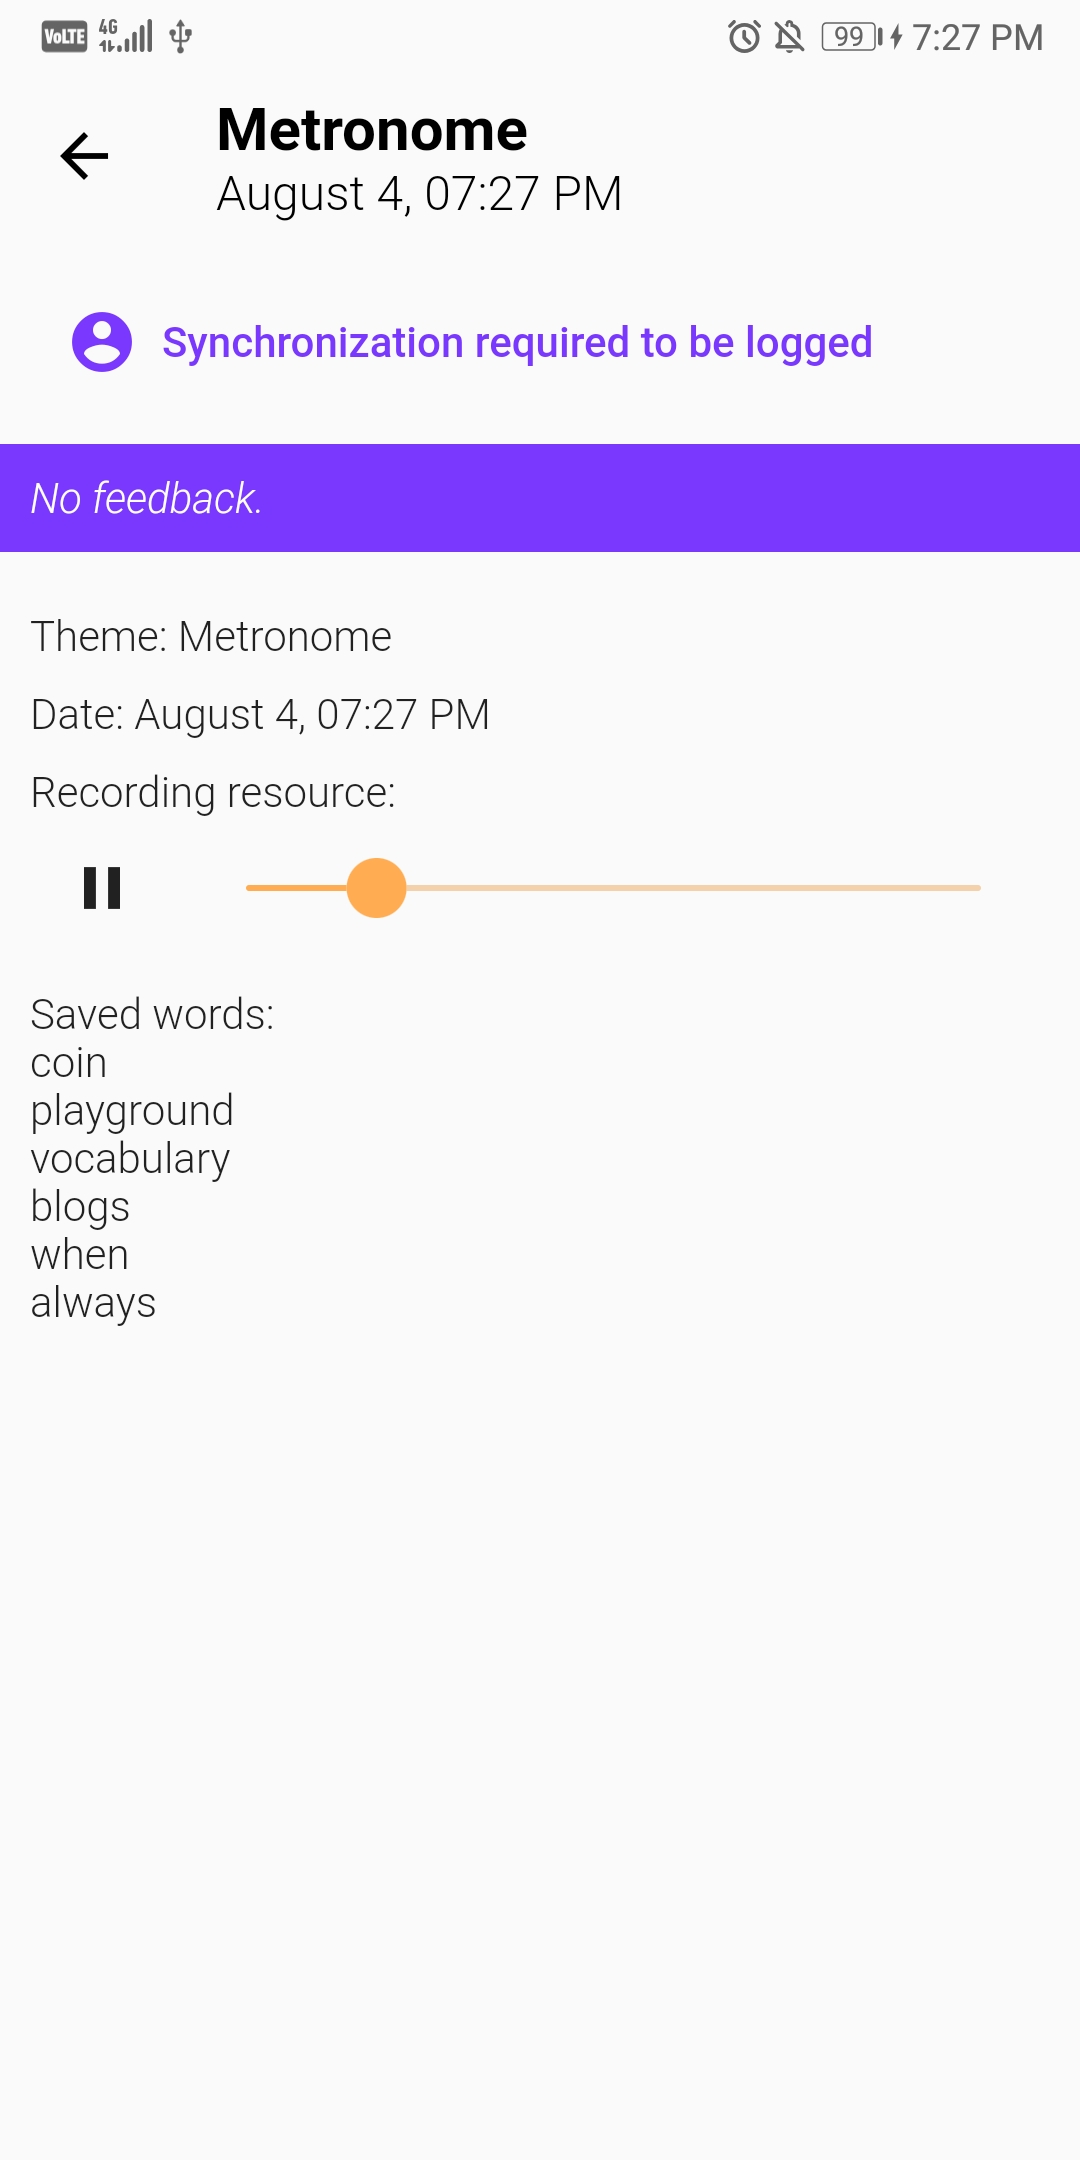
\includegraphics[width=.75\linewidth]{content/imgs/screen6.jpg}
    \caption{Fin de l'exercice, récapitulatif}
    \label{appendix:screen_progress1}
  \end{subfigure}%
  \begin{subfigure}{.25\textwidth}
    \centering
    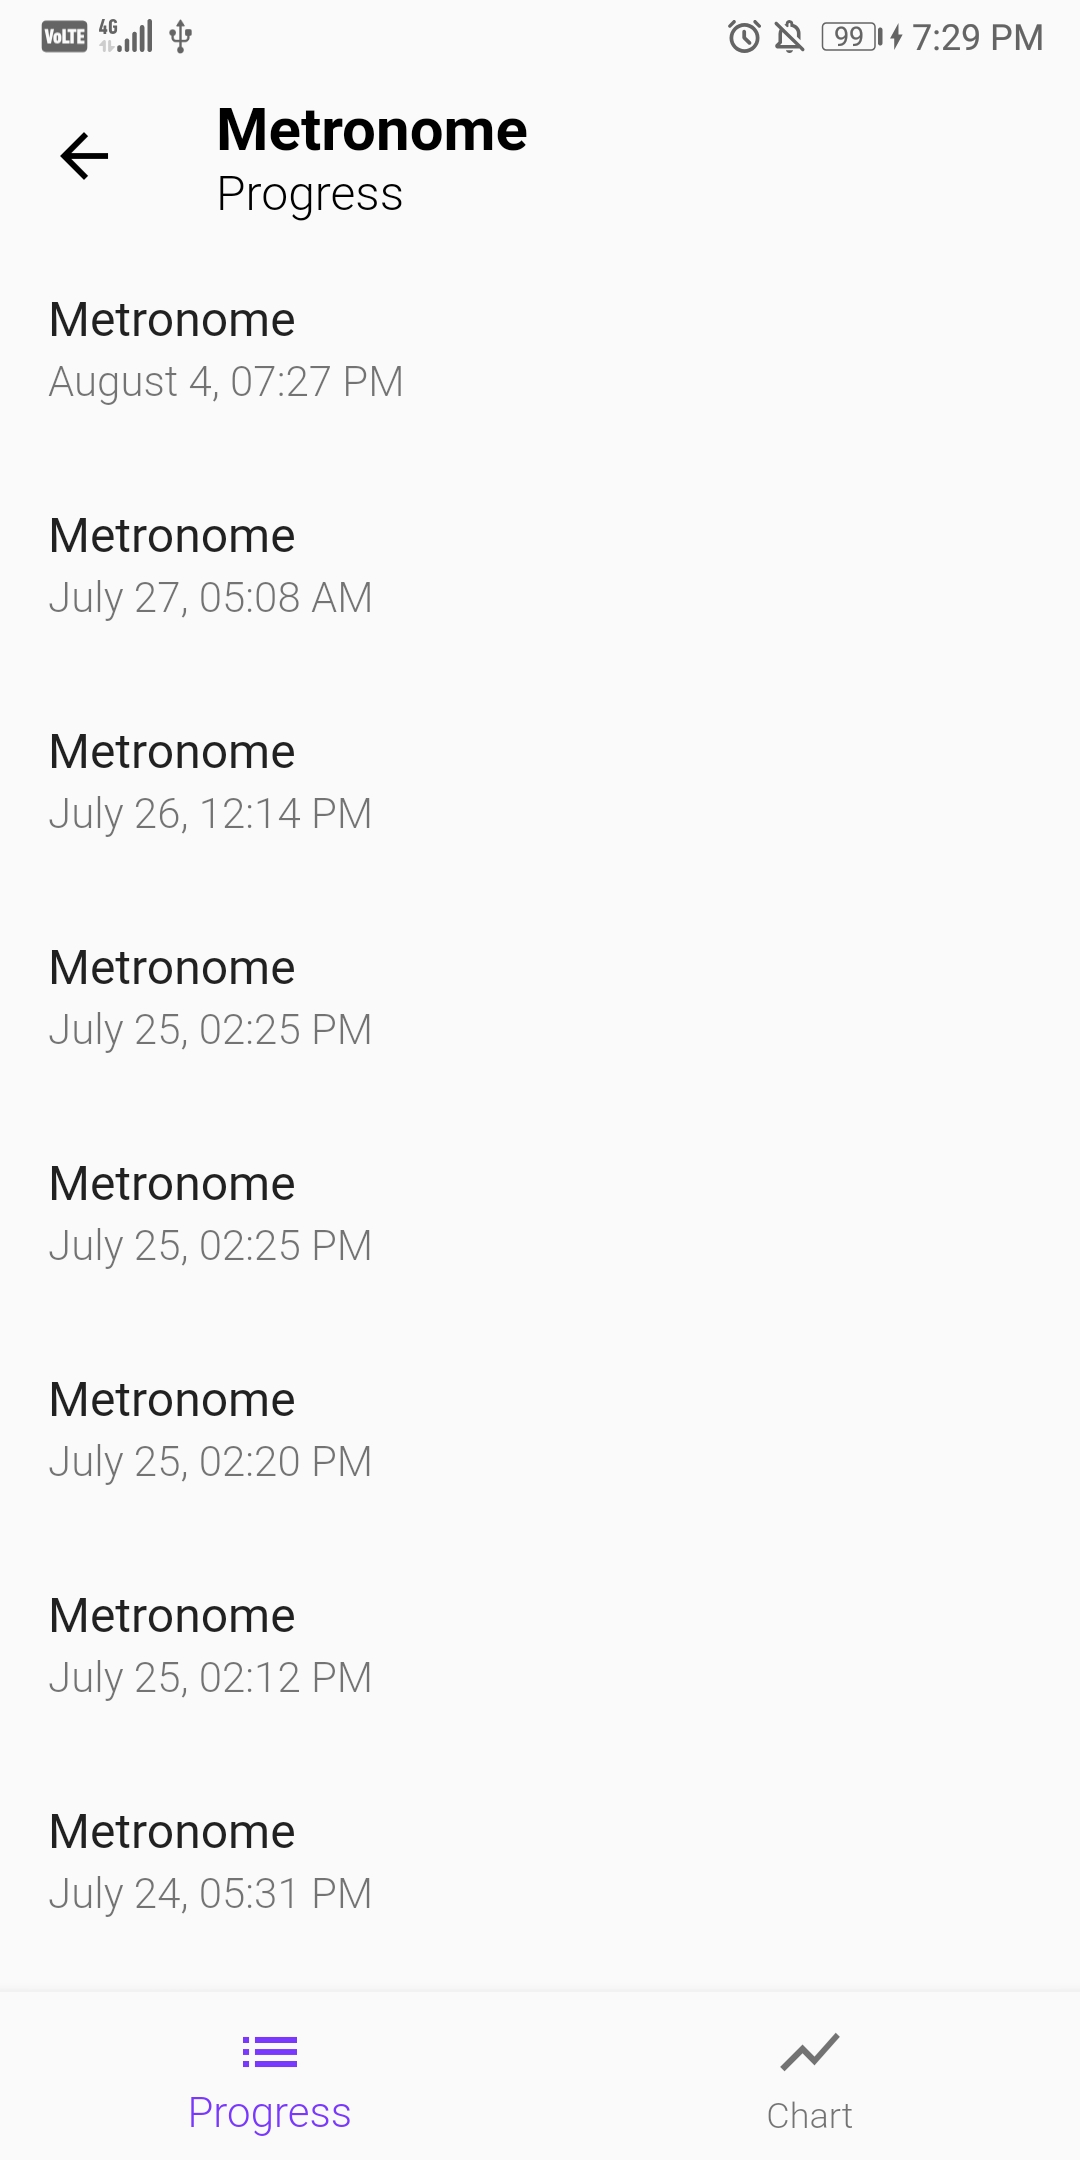
\includegraphics[width=.75\linewidth]{content/imgs/screen7.jpg}
    \caption{Liste de tous les exercices \textit{metronome} effectués}
    \label{appendix:screen_progress2}
  \end{subfigure}%
  \begin{subfigure}{.25\textwidth}
    \centering
    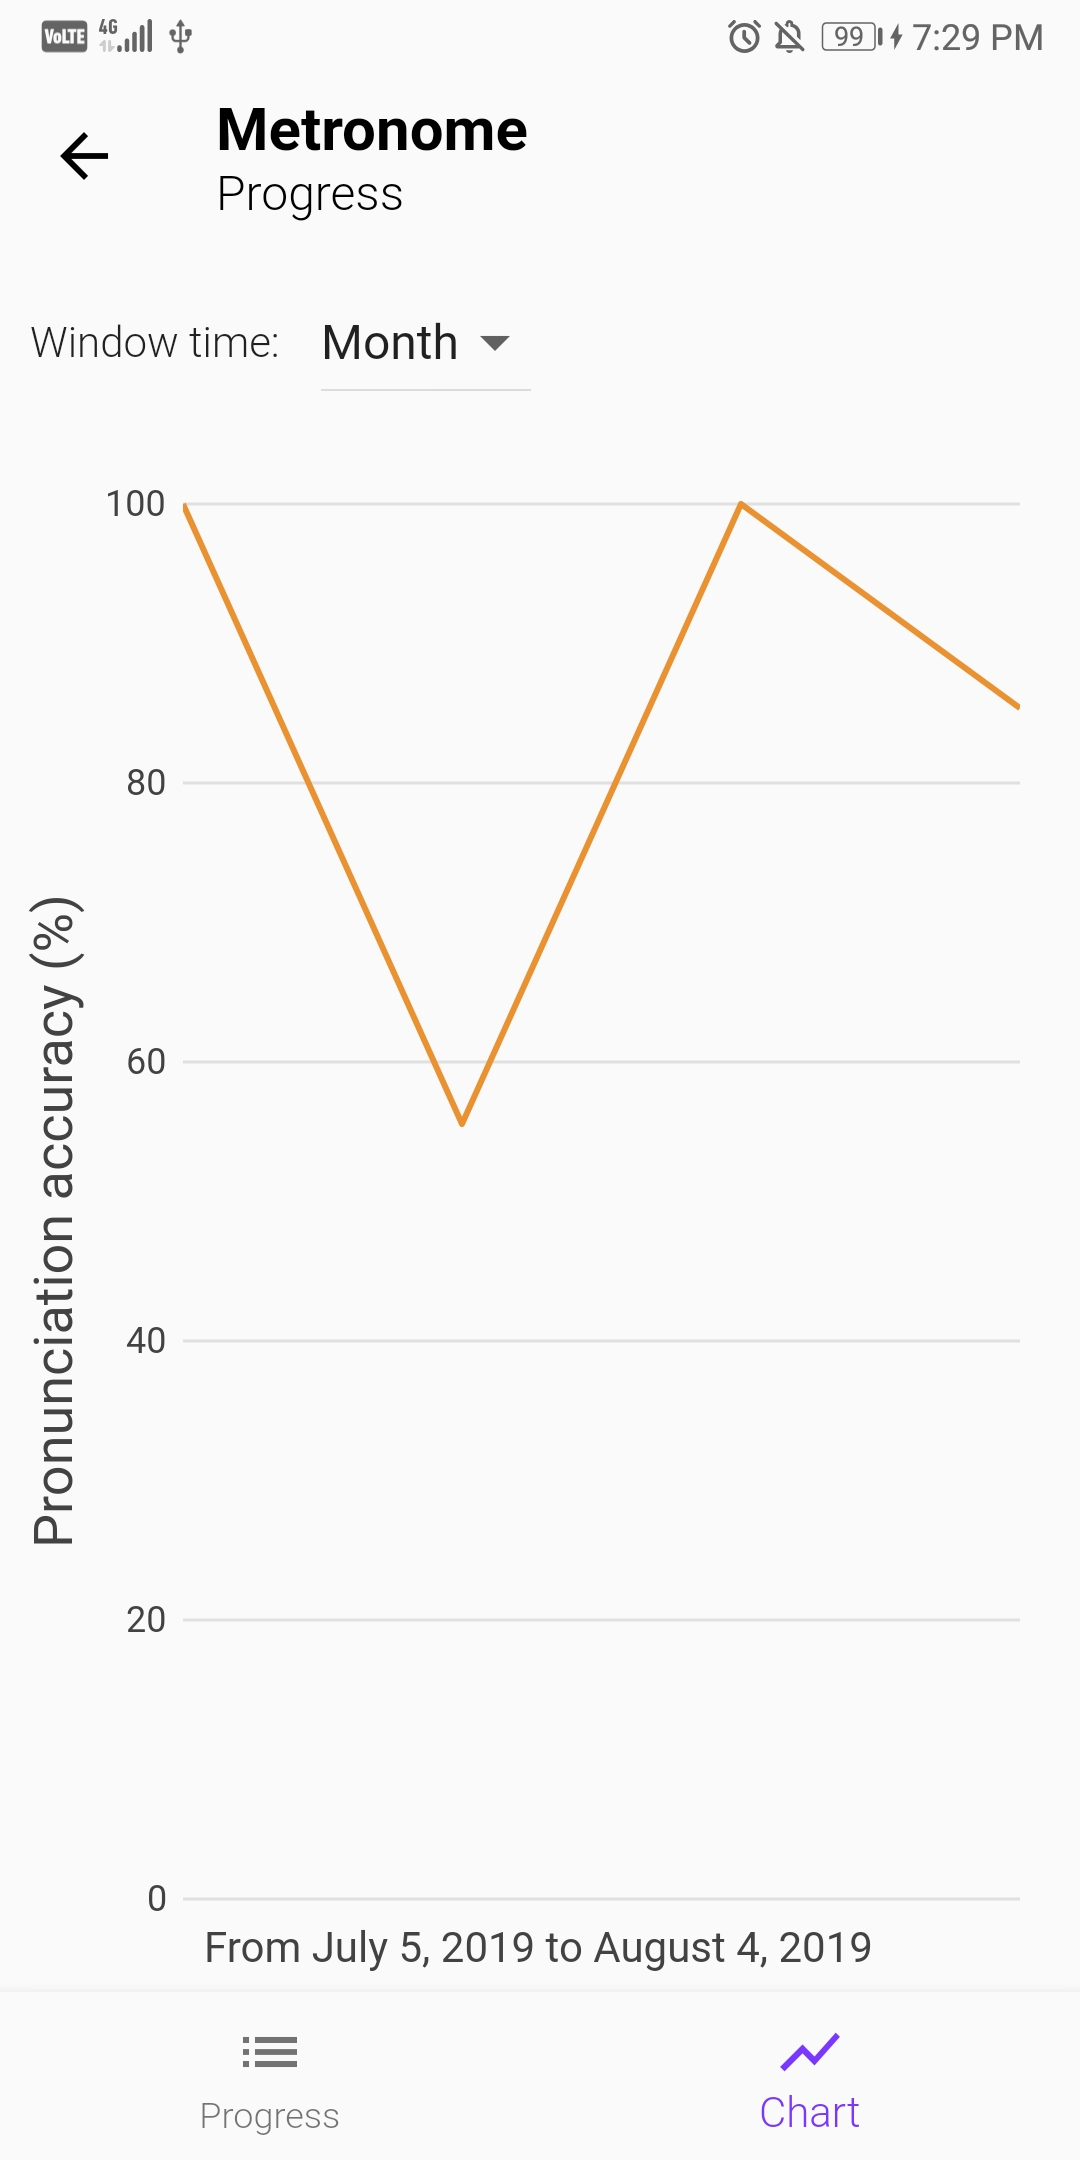
\includegraphics[width=.75\linewidth]{content/imgs/screen8.jpg}
    \caption{Courbe de progression des exercices \textit{metronome}}
    \label{appendix:screen_progress3}
  \end{subfigure}
\end{figure}


\begin{figure}[h]
  \begin{subfigure}{.25\textwidth}
    \centering
    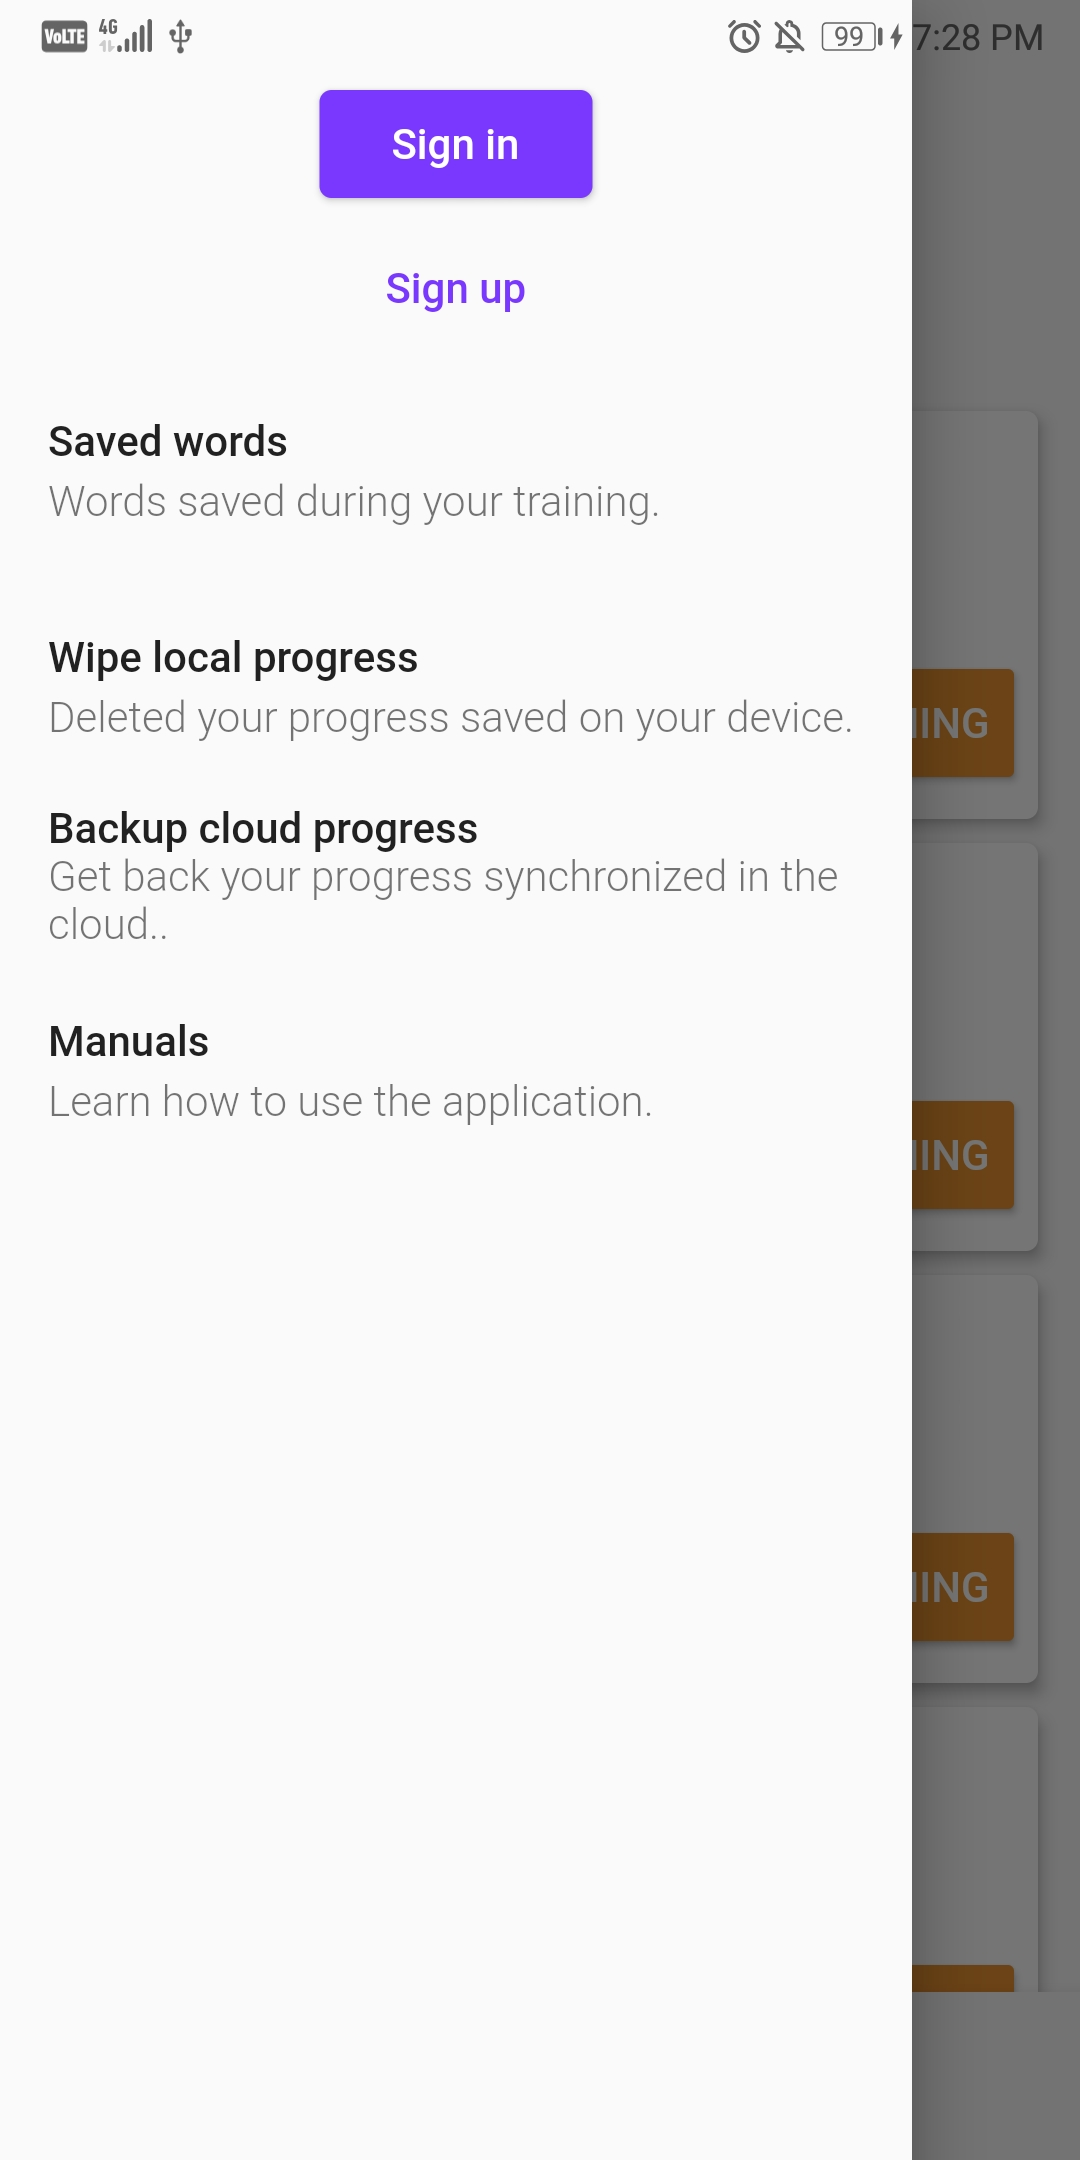
\includegraphics[width=.75\linewidth]{content/imgs/screen9.jpg}
    \caption{Menu de l'application}
  \end{subfigure}%
  \begin{subfigure}{.25\textwidth}
    \centering
    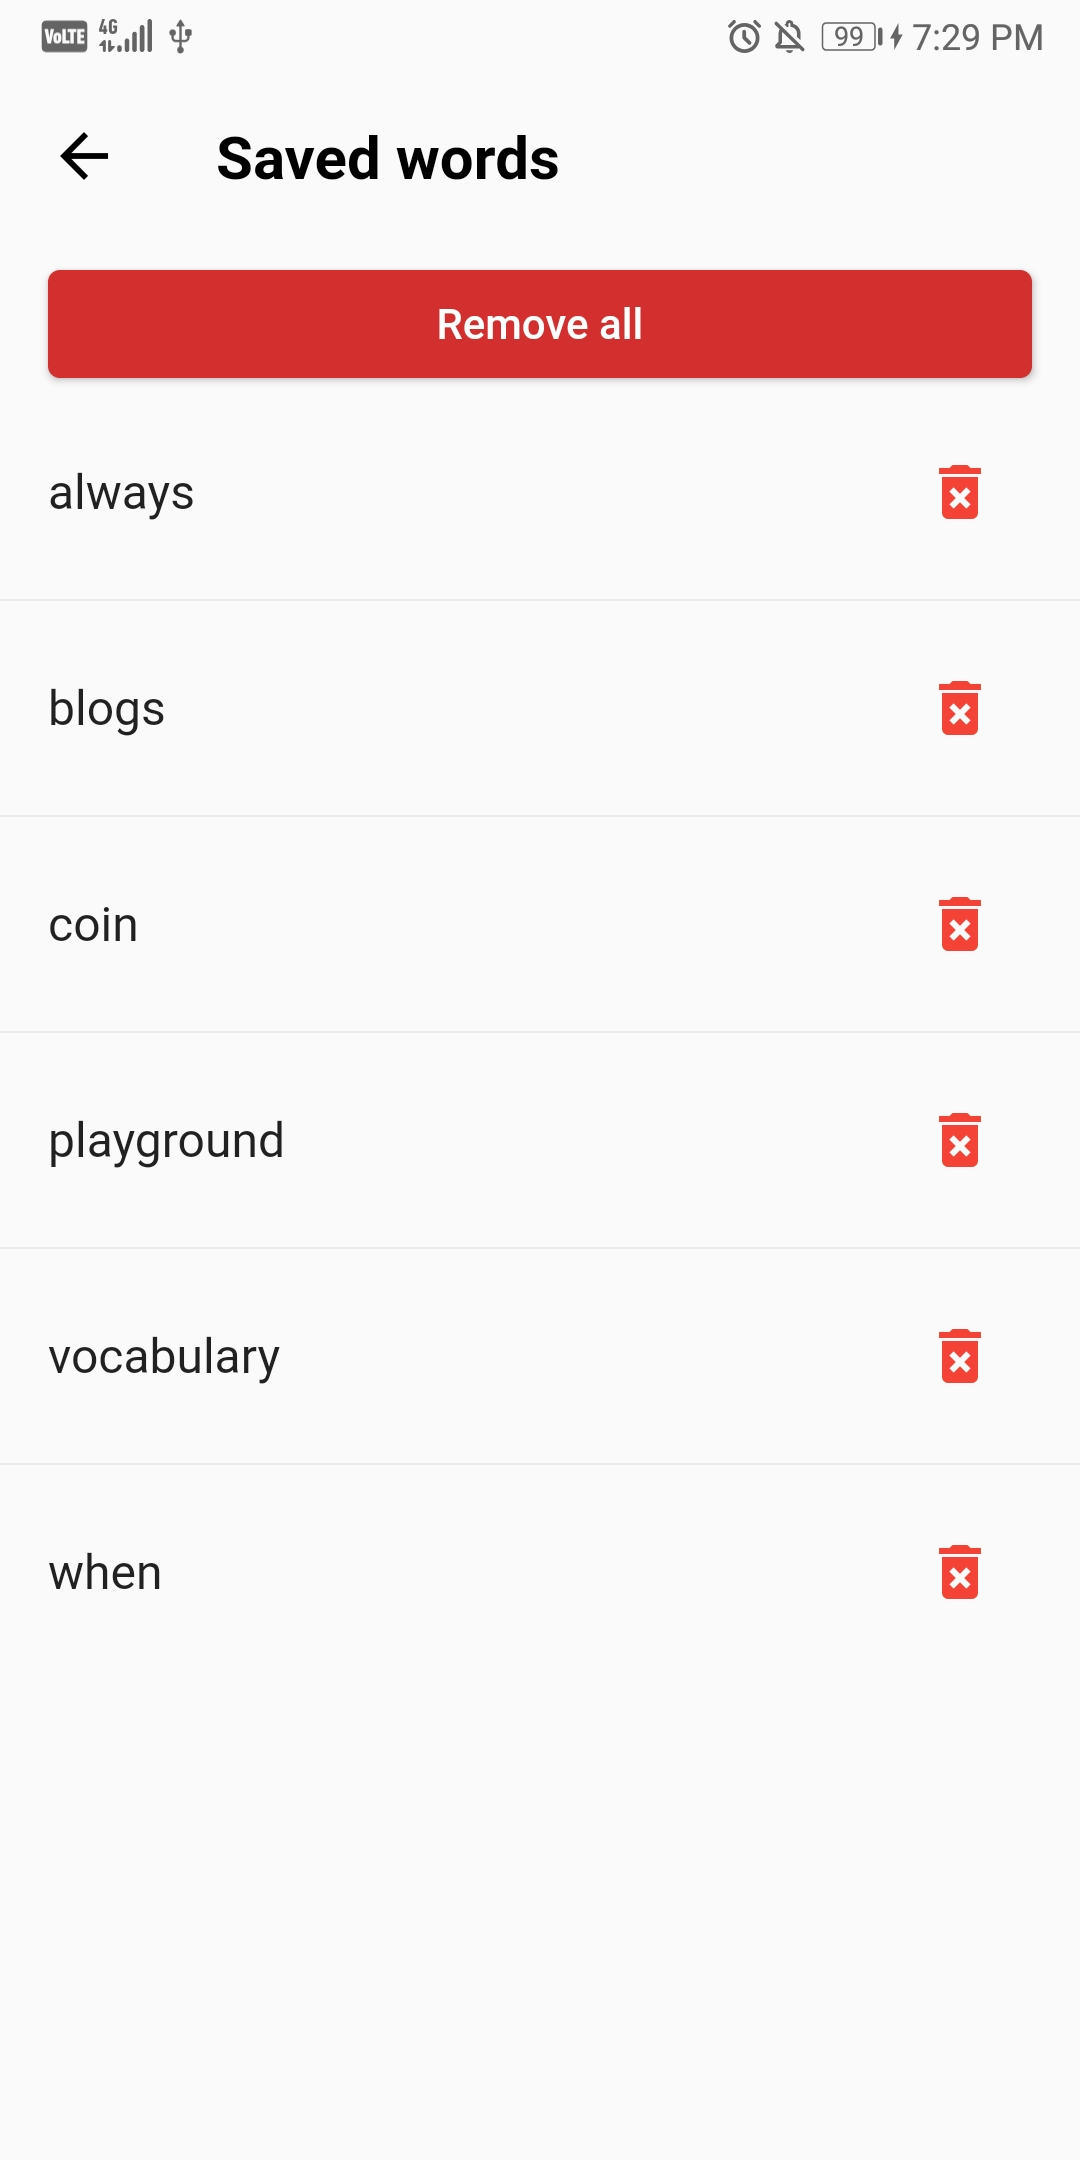
\includegraphics[width=.75\linewidth]{content/imgs/screen10.jpg}
    \caption{Mots mal prononcés lors des exercices}
    \label{appendix:screen_words}
  \end{subfigure}%
  \begin{subfigure}{.25\textwidth}
    \centering
    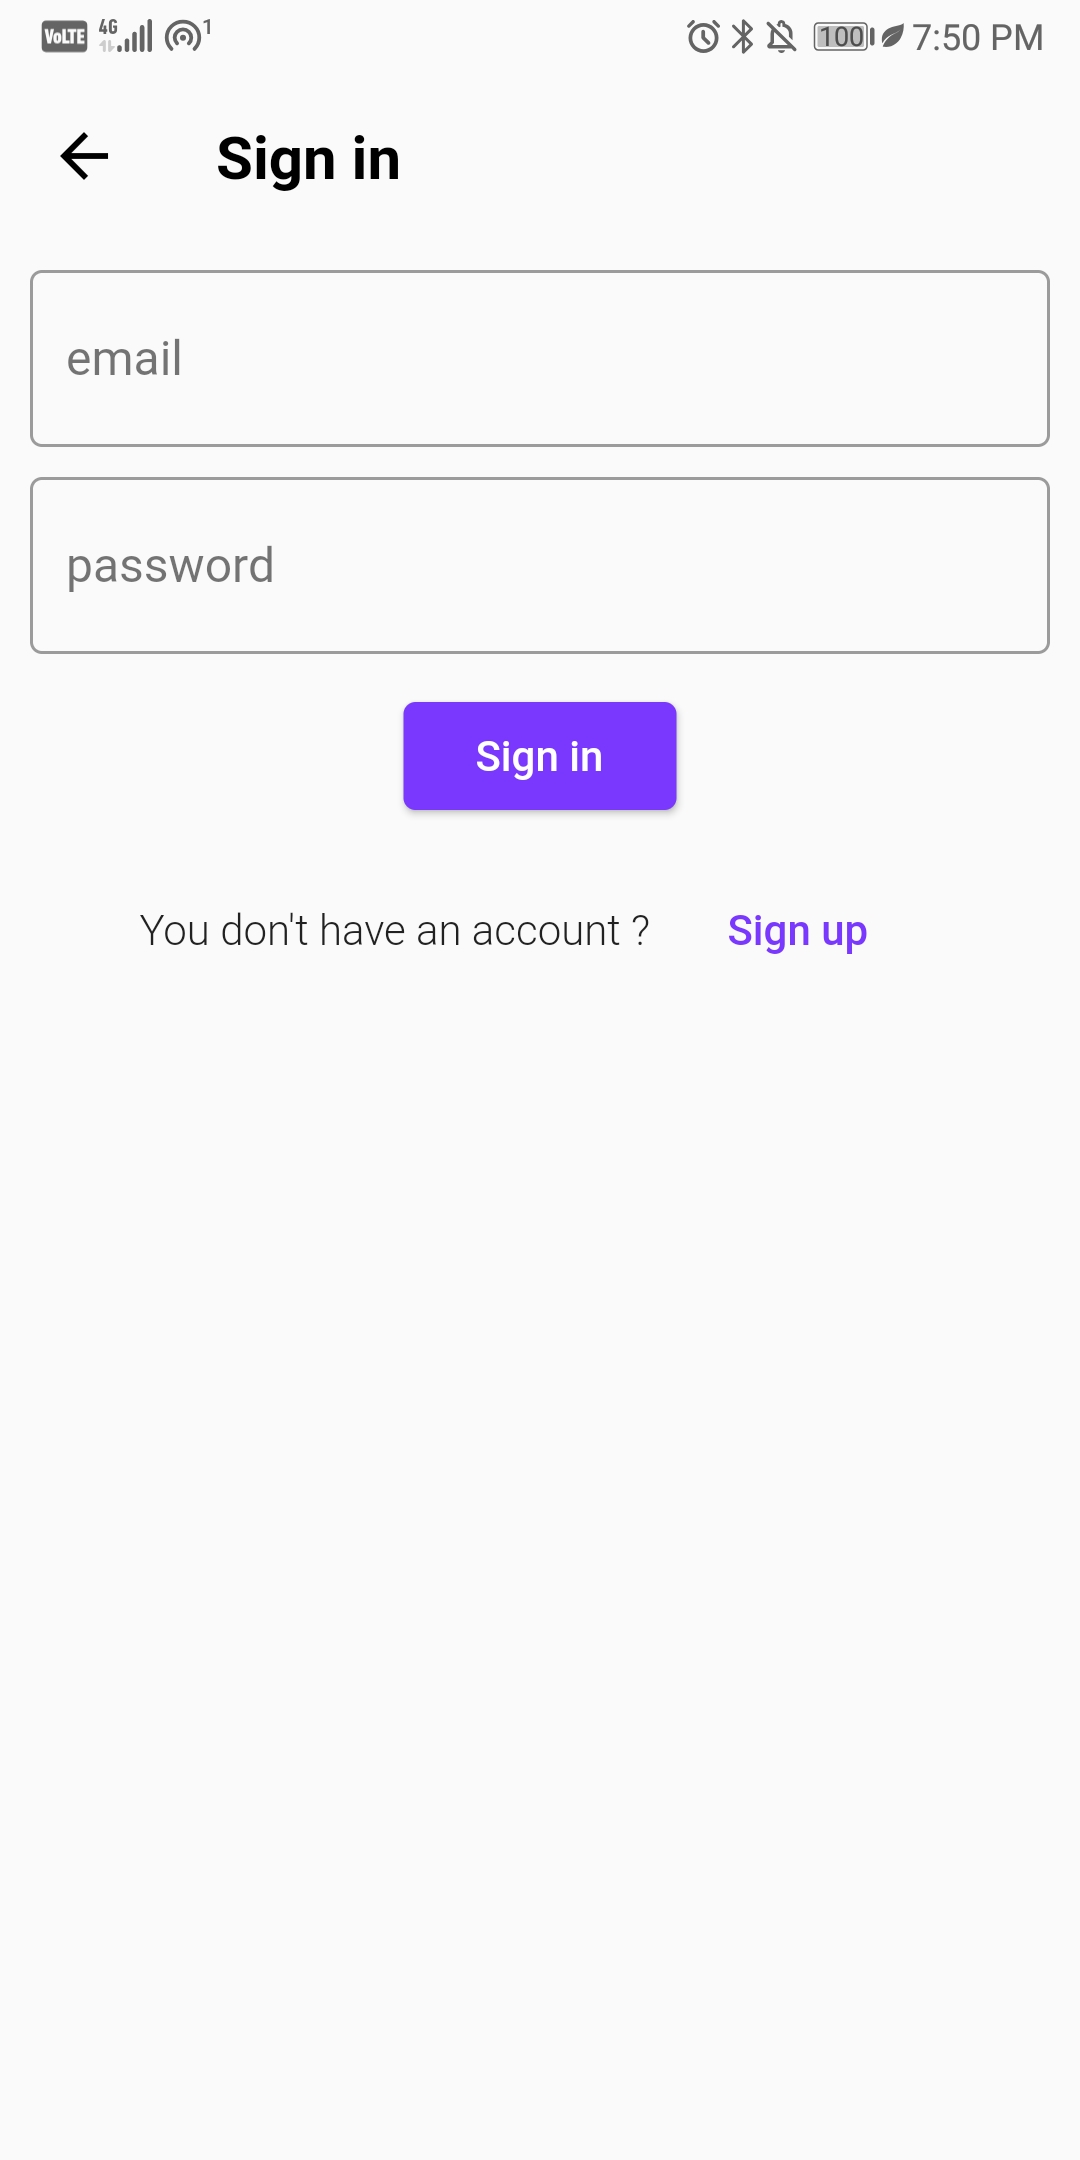
\includegraphics[width=.75\linewidth]{content/imgs/screen11.jpg}
    \caption{Formulaire de connexion}
    \label{appendix:screen_log}
  \end{subfigure}%
  \begin{subfigure}{.25\textwidth}
    \centering
    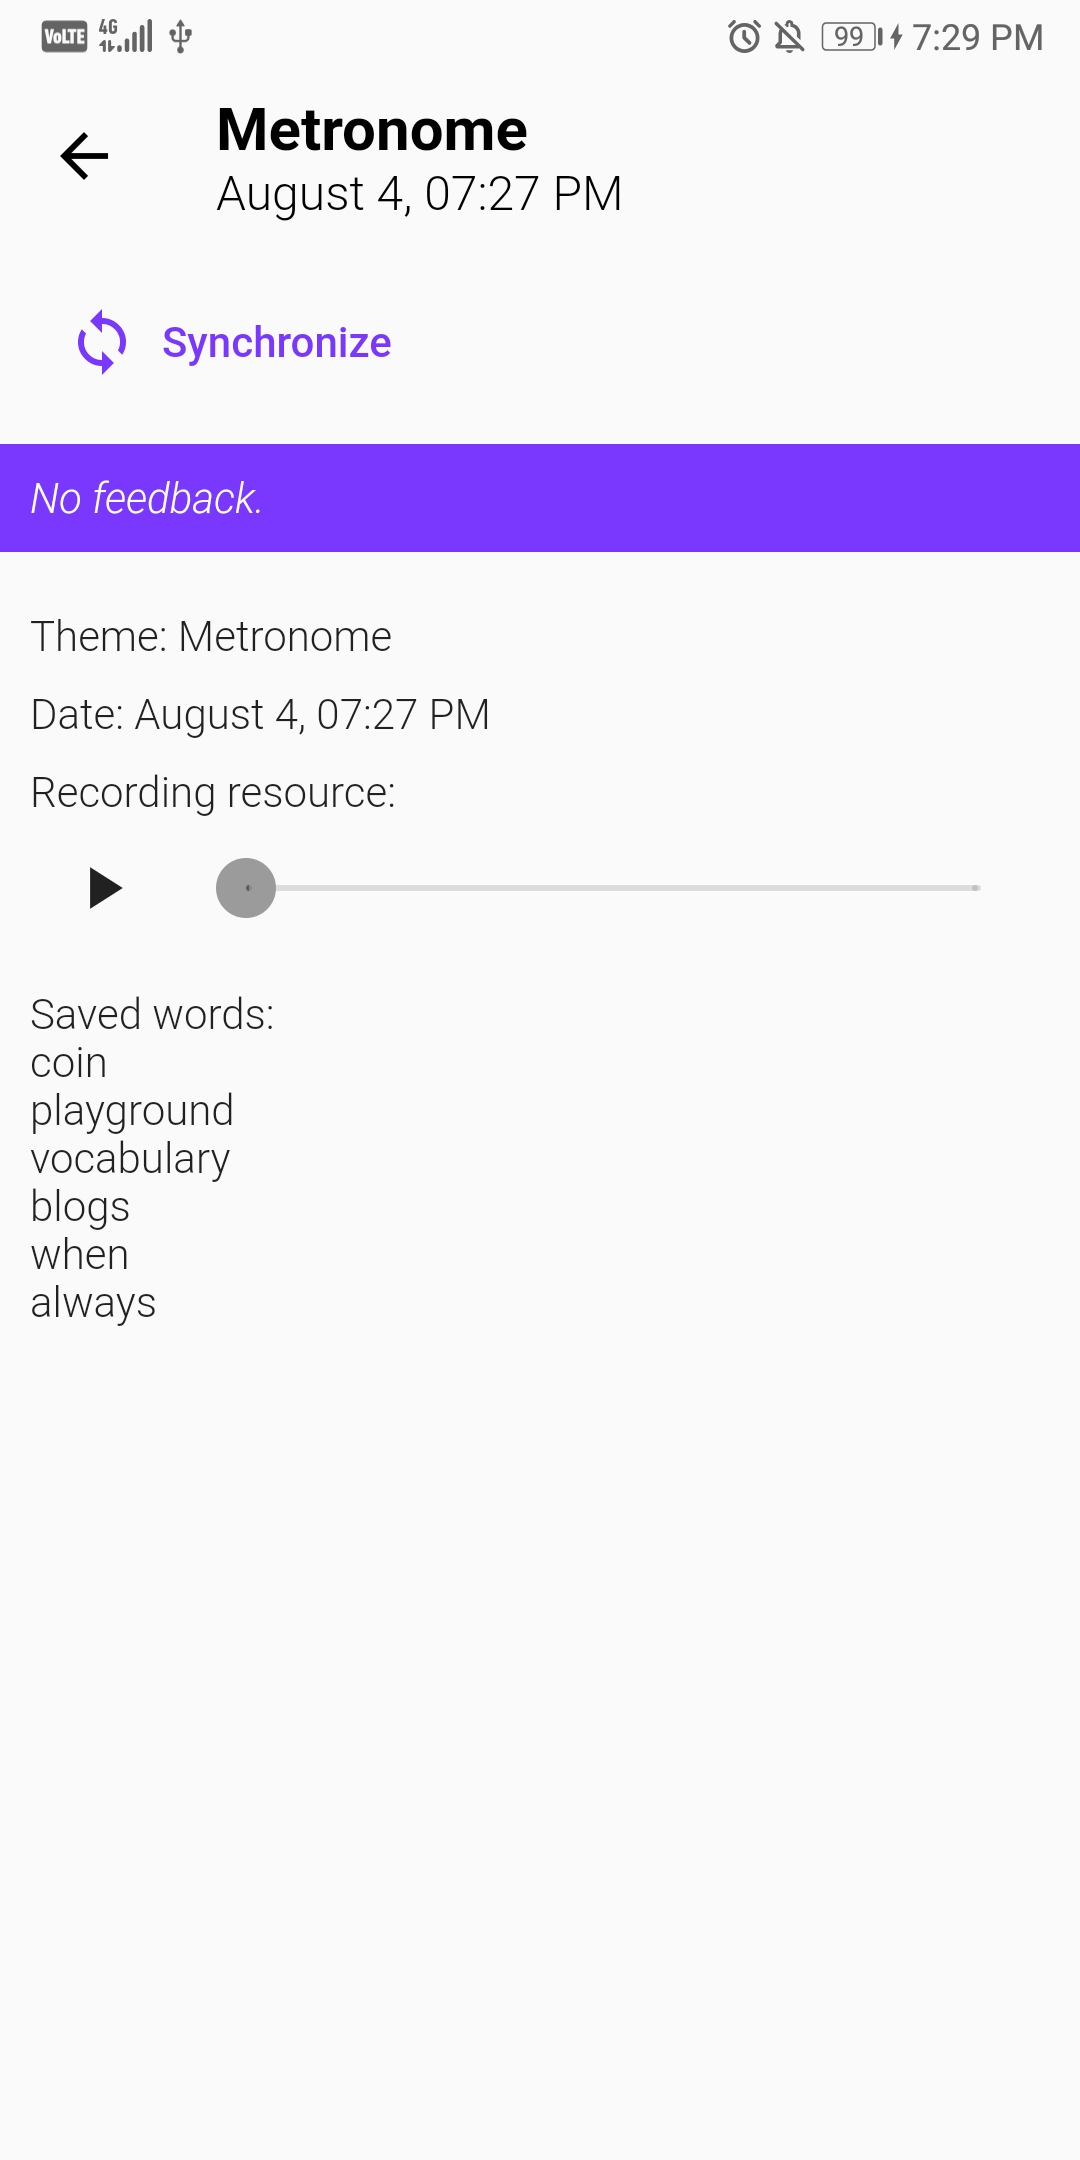
\includegraphics[width=.75\linewidth]{content/imgs/screen12.jpg}
    \caption{Historique d'un exercice avec synchronisation possible}
    \label{appendix:screen_sync}
  \end{subfigure}
\end{figure}


\begin{figure}[h]
  \begin{subfigure}{.25\textwidth}
    \centering
    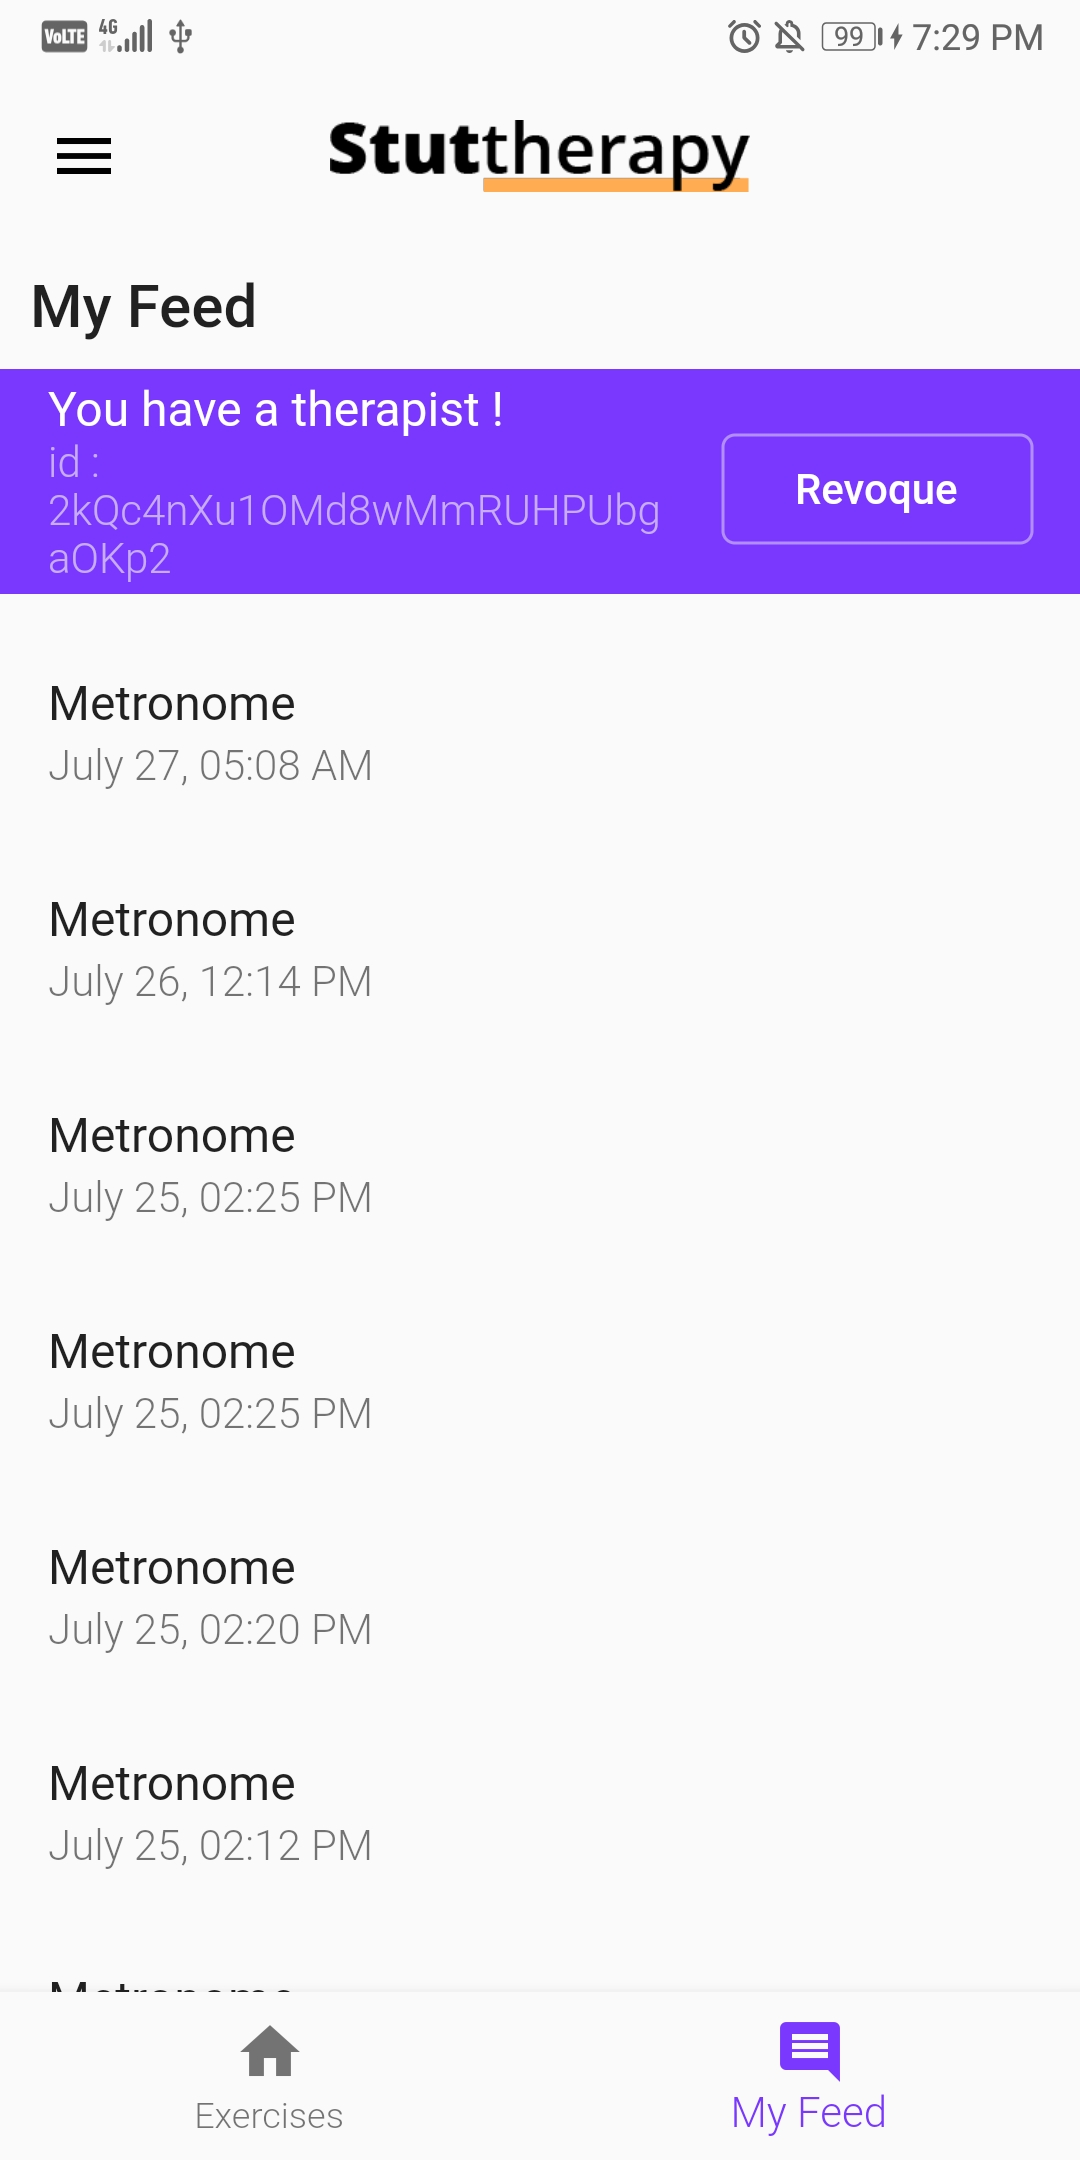
\includegraphics[width=.75\linewidth]{content/imgs/screen13.jpg}
    \caption{Données synchronisées avec un orthophoniste}
    \label{appendix:screen_add_therapist}
  \end{subfigure}%
  \begin{subfigure}{.25\textwidth}
    \centering
    
\includegraphics[width=.75\linewidth]{content/imgs/screen14.jpg}
    \caption{Page d'accueil d'un orthophoniste}
    \label{appendix:screen_therapist1}
  \end{subfigure}%
  \begin{subfigure}{.25\textwidth}
    \centering
    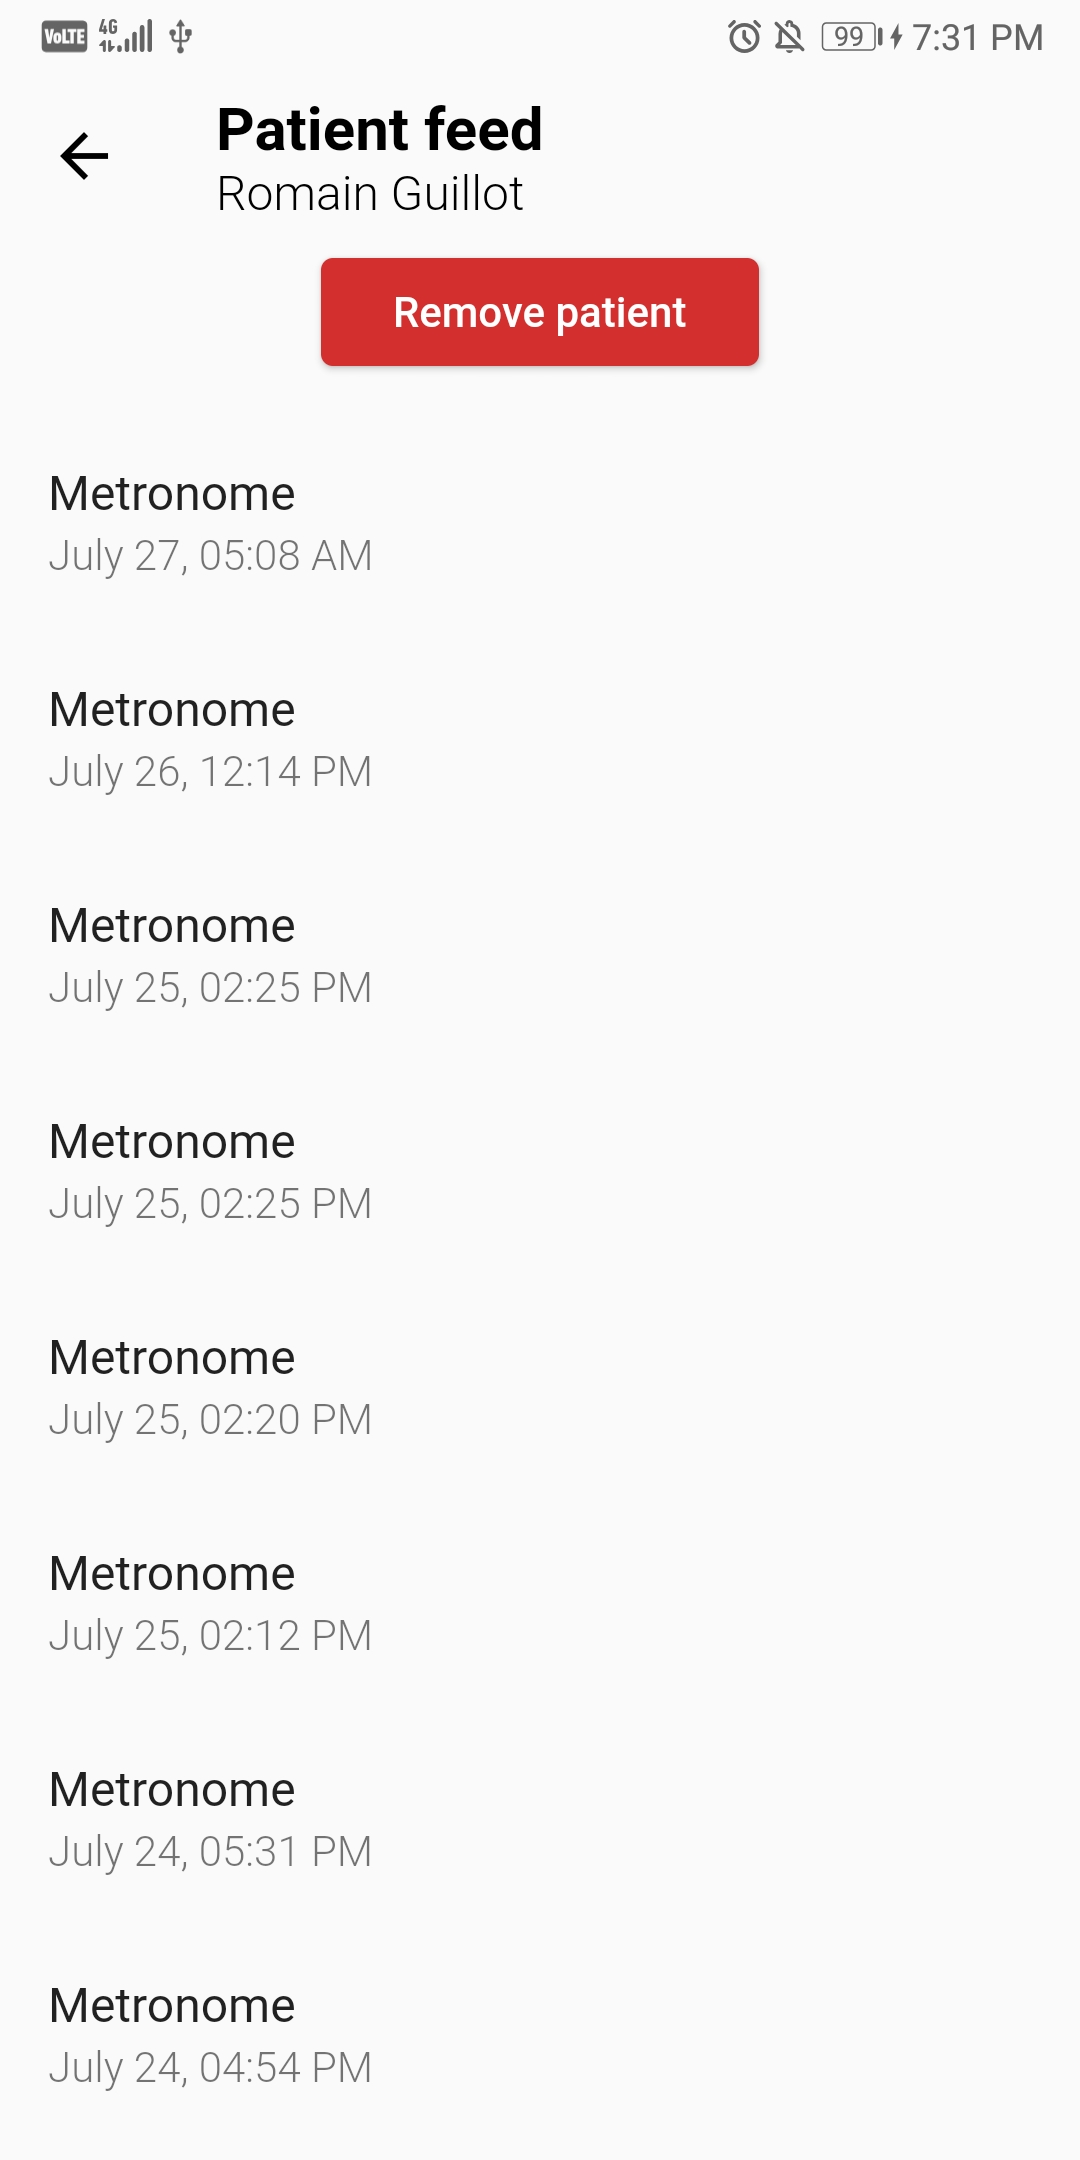
\includegraphics[width=.75\linewidth]{content/imgs/screen15.jpg}
    \caption{Progression d'un patient vu par son orthophoniste}
    \label{appendix:screen_therapist2}
  \end{subfigure}%
  \begin{subfigure}{.25\textwidth}
    \centering
    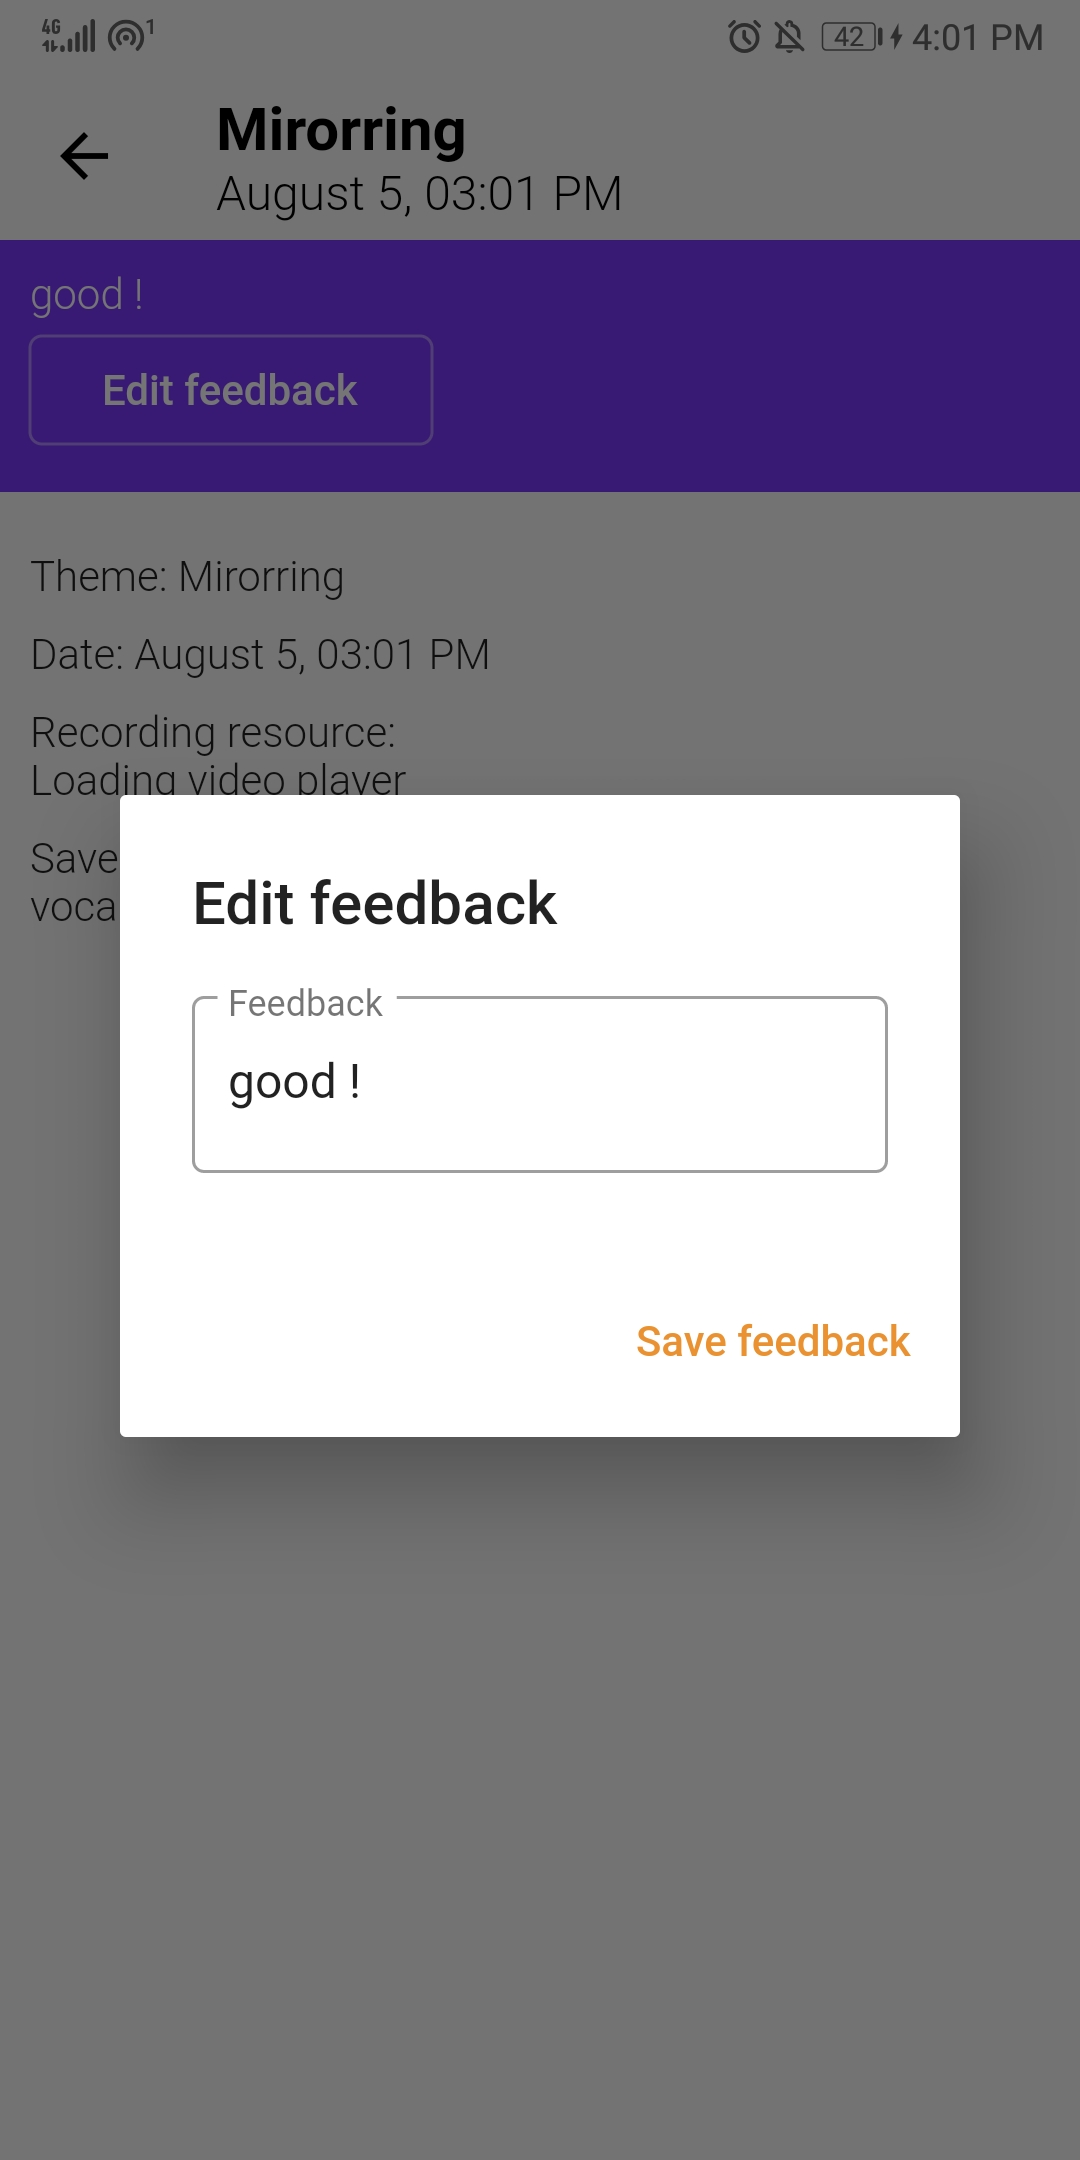
\includegraphics[width=.75\linewidth]{content/imgs/screen18.jpg}
    \caption{Ajout d'un feedback par un orthophoniste}
    \label{appendix:screen_therapist3}
  \end{subfigure}


  \caption*{Captures d'écran de Stuttherapy}
\end{figure}

\begin{figure}[h]
  \begin{subfigure}{.25\textwidth}
    \centering
    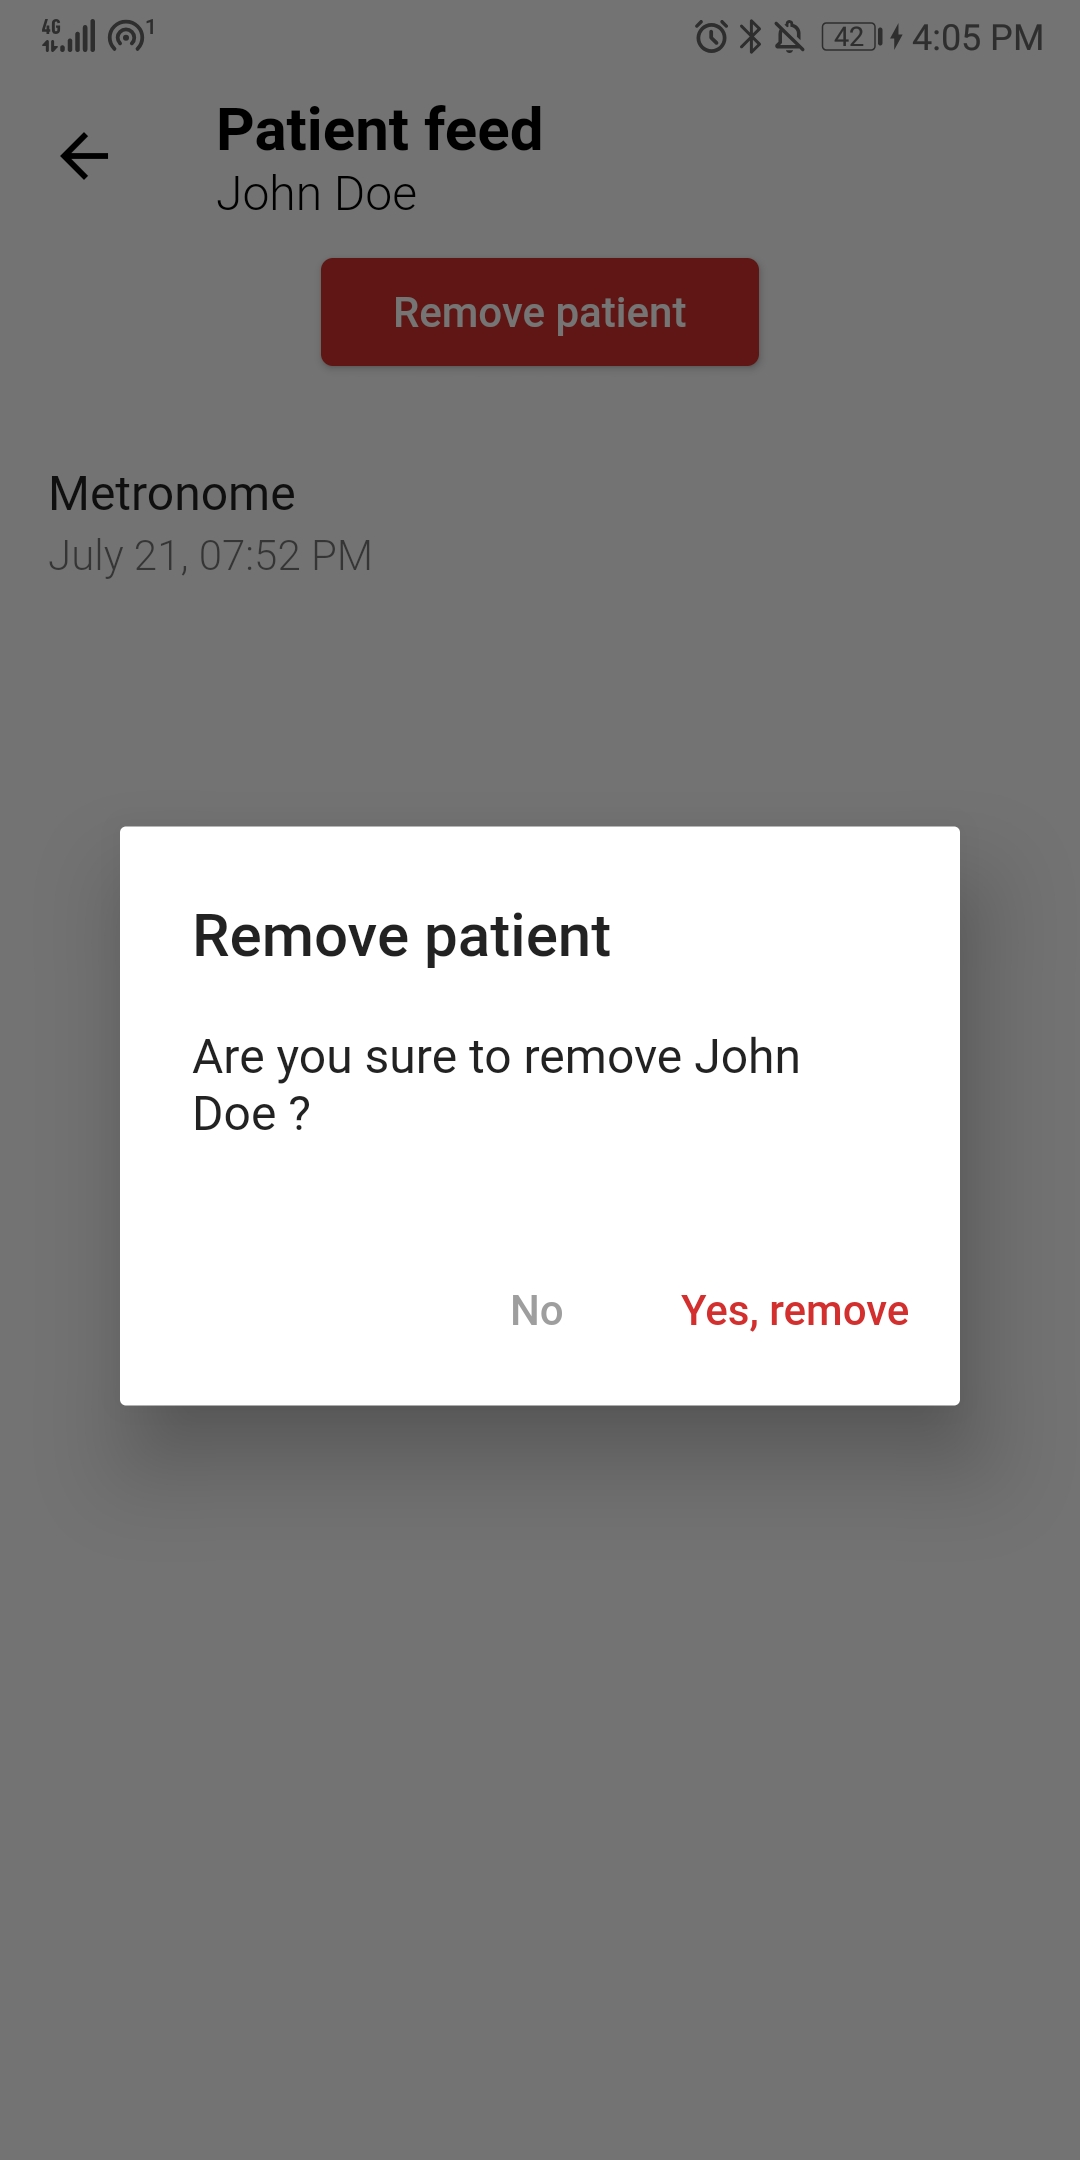
\includegraphics[width=.75\linewidth]{content/imgs/screen19.jpg}
    \caption{Suppression d'un patient}
    \label{appendix:screen_therapist4}
  \end{subfigure}%
  \begin{subfigure}{.25\textwidth}
    \centering
    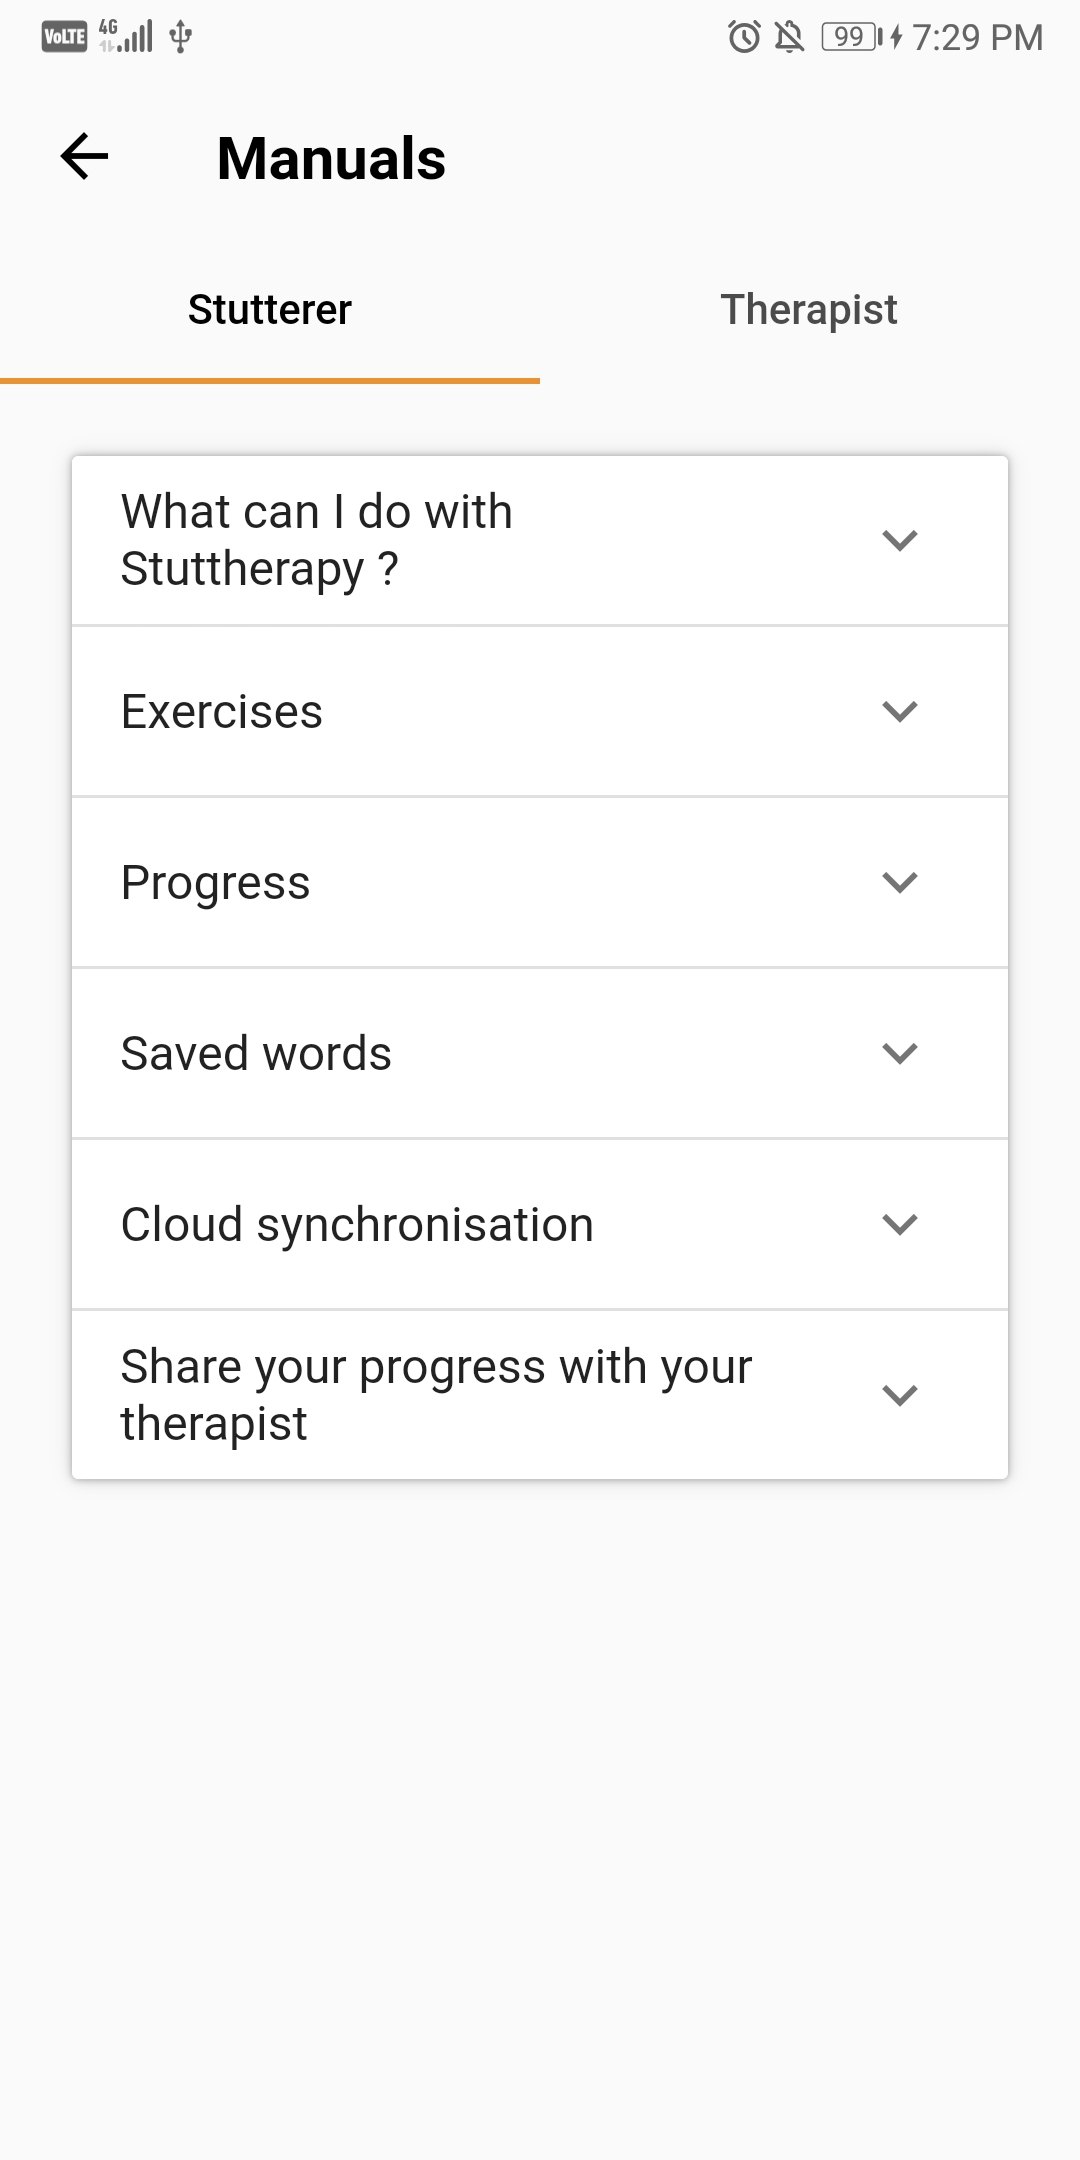
\includegraphics[width=.75\linewidth]{content/imgs/screen16.jpg}
    \caption{Guide pour utiliser l'application}
  \end{subfigure}
\end{figure}

\end{landscape}




\end{appendices}
